% !TeX root=_main_.tex
% chapter5

\chapter{ارزیابی روش پیشنهادی}\label{ch:5}
\thispagestyle{empty}

\epigraph{
«من شکست نخورده‌ام. من فقط $10,000$ راه پیدا کردم که کار نمی‌کند.»
}
{$ \maltese $ {\large توماس ادیسون}}


\noindent
ما روش پیشنهادی خود را روی قالب فایل \gls{PDF} به‌عنوان یک قالب فایل با ساختار پیچیده و ترکیبی و نرم‌افزار متن‌باز و رایگان
 \lr{MuPDF} \cite{MuPDF2018}
 مورد ارزیابی قرار دادیم. در این فصل به تشریح چیدمان آزمایش‌ها، معیارهای ارزیابی، یافته‌های حاصل از آزمایش‌ها و نتیجه‌گیری‌‌ از آنها می‌پردازیم. هدف علاوه بر اثبات کارایی و خوب بودن روش پیشنهادی، شناسایی و تفکیک پارامترهای مهم در هنگام استفاده از فنون یادگیری ماشینی در آزمون فازی و تولید خودکار داده آزمون است. استفاده از یادگیری ماشینی در آزمون فازی حوزه پژوهشی بدیع و ناشناخته‌ای است.  بنابراین در این فصل معیارهایی را که در هر روش پیشنهادی بایستی مورد ارزیابی قرار بگیرند، نیز مشخص خواهیم نمود. سپس روش پیشنهادی خود را با آنها مورد ارزیابی قرار می‌دهیم. 


\section{مورد مطالعاتی}
  نرم‌افزار
 \lr{MuPDF} \cite{MuPDF2018}
 مجموعه غنی از کتابخانه‌ها، \lr{API}ها و ابزارهای کاربردی برای کار با فایل‌های \gls{PDF} است. این نرم‌افزار مشتمل بر سه قسمت \lr{API}، ابزار \lr{mutool} و ابزار \gls{PDF}خوان است. ابزار \lr{mutool} برای ایجاد و تغییر فایل‌های \gls{PDF} استفاده می‌شود. ابزار \gls{PDF}خوان نیز برای نمایش فایل‌های \gls{PDF} به‌کار می‌رود. بسته نرم‌افزاری کامل، به زبان \lr{C} نوشته شده و در سیستم عامل‌های ویندوز، لینوکس و \lr{Mac} و همچنین اندروید قابل استفاده است. به‌دلیل قابلیت حمل بالا و کاربرد زیادی که دارد، پیدا کردن خطا در آن حائز اهمیت است. در آزمایش‌ها ما ابزار \gls{PDF}خوان نسخه ویندوز را مورد آزمون قرار دادیم. منظور از عبارت \lr{MuPDF} در ادامه این فصل همان ابزار \gls{PDF}خوان است.
 
  
  \lr{MuPDF}
  البته در نسخه‌های جدید قالب‌های فایل دیگری را نیز پشتیبانی می‌کند؛ از جمله قالب‌های  فایل \lr{XPS} و \lr{EPub}. اما قالب فایل \lr{PDF} بدون شک رایج‌ترین قالب اسناد و انتشارات الکترونیکی است که بیشتر مردم از آن استفاده می‌کنند. از این‌رو تضمین کیفیت و امنیت \lr{PDF}خوان‌ها به‌ویژه در تلفن‌های همراه اهمیت دو چندانی دارد. افزون بر آنچه گفته شد قالب فایل \gls{PDF} و نرم‌افزار \lr{MuPDF} تمامی مسائلی را که در بخش \ref{problem_statement} بدان اشاره کردیم، یعنی ساختار پیچیده ورودی، ساختار پیچیده کد و غیره، دارند و از طرفی در فصل \ref{related_work} دیدیم که فازرهای مبتنی بر جابه‌جایی مانند \lr{AFL}  و \lr{AFL}افزوده نتواسته بودند به پوشش کد خوبی حیـن آزمون فازی این نرم‌افزار دست‌یابند. بنابراین انتخاب آنها به‌عنوان مورد مطالعاتی به‌دلایل بالا و نیز در جهت فراهم شدن امکان مقایسه با کارهای پیشین، قابل توجیه است. آزمایش‌ها برای هر قالب فایل و هر نرم‌افزار دیگری به‌نحوی که در ادامه این فصل توضیح داده می‌شود قابل اجرا است. 
  
  
 ساختار قالب فایل \gls{PDF} در پیوست \ref{appendix:1} به‌طور کامل بررسی شده است. بخش عمده این ساختار را اشیای متنی تشکیل می‌دهند. از مدل‌های معرفی شده در بخش \ref{sec:model} برای یادگیری ساختار اشیای متنی استفاده می‌کنیم؛ زیرا یادگیری فایل  \gls{PDF} به‌صورت یکجا با توجه به اینکه قسمت‌هایی از آن برای آدرس‌دهی استفاده می‌شوند امکان‌پذیر نیست. اما \lr{MuPDF} یا هر \gls{PDF}خوان دیگری فایل‌های کامل \gls{PDF} را به عنوان ورودی می‌پذیرد به همین لازم است تا اشیای تولید شده را به یک فایل تبدیل کنیم. برای این کار اشیای جدید را با استفاده از سازوکار توضیح داده شده در پیوست آ در مورد بروزرسانی یک فایل \gls{PDF}، به یک فایل معتبر از پیش موجود، که آن را  \gls{Host} می‌نامیم، اضافه می‌کنیم. در نتیجه یک فایل \gls{PDF} جدید در اختیار خواهیم داشت که ساختار آن معتبر بوده و برخی اشیای آن تغییر داده شده و بازنویسی شده‌اند.
 
 
 
 \section{معیارهای ارزیابی}
 در تولید خودکار داده آزمون به روش یادگیری ژرف، تعداد زیادی پارامتر وجود دارد که می‌توان تأثیر آنها را در فرایند آزمون فازی سنجید. اما مهم‌ترین هدف در فرایند آزمون فازی همان‌گونه که پیش از این هم ذکر شد یافتن خطا در \gls{SUT} است. هدف مهم بعدی افزایش میزان پوشش کد برای نیل هر چه بیشتر به هدف اول است. هدف دیگر که مختص به این روش است یادگیری هر چه بهتر ساختار فایل ورودی است. براساس اهداف اشاره شده، معیارهای ارزیابی زیر را در این فصل لحاظ کرده‌ایم:
 \begin{itemize}
 	\item {
 		\textbf{خطا و دقت مدل‌های یادگیری ژرف.}
 	 شامل خطا و دقت هر مدل‌ روی مجموعه‌های آموزش و ارزیابی، میزان و نحوه تغییر آنها با گذشت زمان. این معیارها توسط کد نوشته شده به ابزار \lr{Tensorboard} گزارش شده و در حین فرایند آموزش یا در پایان آن قابل مشاهده هستند.
 
}
	\item {
	\textbf{سرگشتگی.}
	برای ارزیابی میزان خوب بودن مدل زبانی در پیش‌بینی نشانه بعدی توالی داده شده. معیار سرگشتگی از رابطه \ref{ppl} و با جایگذاری خطای مدل روی مجموعه ارزیابی، برای آن مدل محاسبه می‌گردد.
	
}

\item {
	\textbf{پوشش کد.}
	در هر اجرای \gls{SUT}، تعداد خطوط برنامه و نیز تعداد بلوک‌های اولیه‌ای که اجرا شده‌اند، شمارش می‌شود. با داشتن کل خطوط و بلوک‌های اولیه درصد پوشش کد نیز قابل محاسبه است. برای یک مجموعه آزمون، یعنی چندین بار اجرای متوالی \gls{SUT} پوشش کد عبارت خواهد بود از اجتماع پوشش کد تک‌تک هریک از اجراها. بنابراین منظور از اصطلاح کلی پوشش کد در ادامه پوشش بلوک‌های پایه است.  
	
}
\item {
\textbf{خطا و آسیب‌پذیری.}
\gls{SUT}
تحت ابزار پایش \lr{Application Verifier} اجرا می‌شود که خطاهای احتمالی را ثبت و شماره‌گذاری می‌کند. سپس می‌توان با تحلیل این خطاها در یک محیط اشکال زدا، ضمن تعیین مکان و علت خطا، امکان قابل بهره‌برداری بودن آنها را بررسی کرد.
}
 \end{itemize}

آزمایش‌ها بایستی به‌گونه‌ای طراحی شوند که هریک از آنها تأثیر یک پارامتر خاص را بر روی معیارهای بالا، به‌طور واضح نمایان سازد؛ اما، پارامـــترها کدامند؟ ما در این بخش، چندین پارامتر و مقادیر قابل آزمایش برای هریک را شناسایی و معرفی می‌کنیم. فهرستی از این پارامترها و مقادیری که می‌توانند بپذیرند در جدول \ref{tabel:all_parameters} ذکر شده است. همان‌طور که مشاهده می‌شود برخی از پارامترها مقادیری پیوسته و برخی دیگر مقادیری گسسته می‌پذیرند. بر این باور هستیم که هر روش تولید خودکار داده آزمون با استفاده از یادگیری ماشینی روی چنین پارامترهایی بنا می‌شود، لذا شناسایی و تفکیک این پارامترها پیش از هرگونه طرح آزمایشی لازم و ارزشمند است.

\begin{table}%[ht]
	\caption[پارامترهای مؤثر در تولید خودکار داده آزمون با روش‌های یادگیری ماشینی و مقادیر قابل آزمایش برای آنها]{
		پارامترهای مؤثر در تولید خودکار داده آزمون با روش‌های یادگیری ماشینی و مقادیر قابل آزمایش برای آنها.}
	\label{tabel:all_parameters}
	\centering
	\onehalfspacing
	%\setlength{\extrarowheight}{4mm}
	\begin{tabularx}{0.95\linewidth}{rrr}
		\toprule[1.5pt]
		 ردیف  &
		 پـارامتـر \hspace{2cm} &
		 مقادیر قابل آزمایش 
		\\
		\midrule[1.5pt] 
		1 &
		 نوع مدل & 
		$\bullet$
		 انواع مدل‌های یادگیری ژرف 
		\\
		\hline
		 2 &
		 راهبرد & 
		 $\bullet$
		 حریصانه 
		 \\
		  &
		  &  
		  $\bullet$
		  نمونه برداری
		 \\
		  &
		  &  
		  $\bullet$
		  ترکیبی (حریصانه + نمونه‌برداری) 
		 \\
		  &
		  &  
		  $\bullet$
		  چند فهرست بهتر 
		 \\
		\hline
		%\vspace{3mm}
		 3 &  تنوع 
		 ($D$) & 
		 $\bullet$ $(0, \infty)$
		\\
		\hline
		%\vspace{3mm}
		 4 &
		 روش فاز &
		 $\bullet$
		 بدون فاز 
		 \\
		  &
		  &
		 $\bullet$
		 تصـادفی
		 \\
		  &
		 &
		 $\bullet$
		 مبتنی بر مدل 
		 \\
		  &
		  &
		  $\bullet$
		 ترکـیبی
		 \\
		\hline
		%\vspace{3mm}
		5 & 
		الگوریتم فاز & 
		$\bullet$
		فاز داده
		\\
		&
		&
		$\bullet$
		فاز فراداده 
		\\
		\hline
		%\vspace{3mm}
		 6 &  تعداد دوره آموزش & 
		 $\bullet$ $\{1,2,3,...\}$
		\\
		\hline
		%\vspace{3mm}
		7 &
		نوع فایل &
		$\bullet$
		متنی
		\\
		&
		&
		$\bullet$
		متنی + دودویی
		\\
		\hline
		%\vspace{3mm}
		8 &
	
		استفاده از میزبان &
		$\bullet$
		استفاده
		\\
		&
		&
		$\bullet$
		عدم استفاده 
		\\
		\hline
		%\vspace{3mm}
		 9 &  تعداد میزبان & 
		 $\bullet$ $\{1,2,3,...\}$
		\\
		\hline
		10 &
		میزان تغییر میزبان &
		$\bullet$
		ثابت
		\\
		&
		&
		$\bullet$
		متغیر
		\\
		\bottomrule[1.5pt]	
	\end{tabularx} 
\end{table}
 
 نوع مدل در سطر اول جدول \ref{tabel:all_parameters} برای هر مدل، خود دارای اَبَرپارمترهایی مانند تعداد عصب، لایه، نرخ یادگیری و غیره است که در فصل قبل به آنها اشاره شد. بنابراین جدول \ref{tabel:all_parameters} یک دید جامع از همه پارامترهایی که تا اینجا معرفی شدند، در اختیار می‌گذارد. در بخش بعد چیدمان آزمایش‌ها خود را براساس این پارامترها شرح خواهیم داد.
 
 

 \section{چیدمان آزمایش‌ها}
 
  برای آموزش مدل‌های یادگیری معرفی شده در بخش \ref{sec:model} (جدول \ref{tabel:deep_model}) و تولید داده‌های آزمون از یک سیستم فیزیکی با پردازنده گرافیکی 
  \lr{NVidia GTX 1080}،
  پردازنده مرکزی 
  \lr{Intel Core i7 }
  و 20 گیگابایت حافظه اصلی به همراه سیستم عامل 
  \lr{Ubuntu 16.04 x64}
  استفاده کردیم. آزمون‌های فازی را نیز روی ماشین مجازی با پردازنده 
  \lr{Intel Core i7 } 
  و 8 گیگابایت حافظه اصلی به همراه سیستم عامل 
 \lr{Windows 10 x64}
انجام دادیم. ما همچنین از نسخه نهایی 
\lr{MuPDF}
در زمان انجام آزمایش‌ها یعنی نسخه 
\lr{MuPDF 1.11(2017-04-11) Final}
برای آزمون فازی استفاده کردیم. باتوجه به نهایی بودن نسخه انتظار می‌رود خطاهای نسخه تا حد زیادی، در مقایسه با نسخه‌های آلفا، بتا و 
\lr{RC}
برطرف شده باشند و لذا شناسایی خطا کار سخت‌تری خواهد بود.
مشخصه‌های کامل مدل‌ها در فرایند آموزش به‌همراه تعداد دوره و زمان آموزش هر دوره، در جدول \ref{tabel:model_parameters} آمده است.

\begin{table}%[ht]
	\caption{
		مشخصه‌ها و زمان آموزش مدل‌های جدول \ref{tabel:deep_model} در فرایند آموزش.}
	\label{tabel:model_parameters}
	\centering
	\onehalfspacing
	\begin{tabularx}{0.95\linewidth}{r p{15mm} p{15mm} p{15mm} p{15mm}}
		
		\toprule[1.5pt]  پارامتر / شماره مدل & 1 & 2 & 3 &  4
		\\
		\midrule[1.5pt] طول توالی‌های ورودی ($d$) & 50 & 50 &  50 & 50 
		\\
		%\hline
		 گام پرش ($j$) & 3 & 3 &  1 & 1 
		\\
		%\hline
		 تعداد دوره & 50 & 50 &  50 & 50 
		\\
		%\hline
		 زمان تقریبی یک دوره (ساعت: دقیقه) &   $  1:00'$  &   $1:45'$  &  $5:45'$&           $  9:30'$ 
		\\
		%\hline
		 حجم تقریبی مدل (مگابایت) & $ 1.24$ & $ 2.76$ &  $ 9.99$ & $ 5.41$ 
		\\
		\bottomrule[1.5pt]
		
	\end{tabularx} 
\end{table}
 
 پیچیدگی مدل‌های جدول \ref{tabel:model_parameters} با افزایش شماره، افزایش می‌یابد. یعنی مدل 2 از مدل 1 پیچیده‌تر درنظر گرفته شده است. همان‌طور که در جدول هم مشخص است مدل‌های پیچیده‌تر زمان آموزش طولانی‌تری دارند. برای مدل‌های پیچیده‌تر منطقی است که نمونه‌های آموزشی بیشتری داشته باشیم. در نتیجه برای مدل‌های 3 و 4 گام پرش را 1 و برای مدل‌های 1 و 2 گام پرش را 3 در نظر گرفتیم. همچنین برای مدل شماره 3 از روش منظم‌سازی
 \lr{Dropout} \cite{JMLR:v15:srivastava14a}
   $p=0.3$ 
  استفاده کردیم. در نهایت هر مدل را دست‌کم برای $50$ دوره روی داده‌های مجموعه آموزش، آموزش دادیم.
 
 \subsection{مجموعه داده}
 آموزش موفق شبکه‌های عصبی ژرف مستلزم داشتن مجموعه داده به‌اندازه کافی بزرگ و مناسب است. در یادگیری ماشینی هرچه‌قدر تعداد داده‌ها بیشتر باشد، یادگیری بهتر انجام خواهد شد. هنوز در بسیاری از زمینه‌ها مجموعه داده کافی برای آموزش وجود ندارد و این یکی از محدودیت‌های استفاده از شبکه‌های عصبی ژرف است. برای یادگیری آماری ساختار اشیای فایل \gls{PDF} پیکره بزرگی از فایل‌های \gls{PDF} جمع‌آوری کردیم؛ زیرا چنین پیکره‌ای از قبل وجود نداشت. بخشی از این پیکره شامل مجموعه داده‌های آزمون \gls{PDF} خوان
  \lr{Mozilla}\LTRfootnote{\href{https://github.com/mozilla/pdf.js/tree/master/test/pdfs}{https://github.com/mozilla/pdf.js/tree/master/test/pdfs}} 
   است که در مرورگر وب
    \lr{Firfox}
     و دیگر پروژه‌های این شرکت استفاده می‌شود و به‌صورت رایگان دردسترس است. بخش دیگری از آن \gls{PDF}های استفاده شده در فازرهای دیگر مثل
      \lr{AFL}
       است و بلأخره بخشی بزرگی نیز از طریق وب جمع‌آوری شد به‌نحوی که تنوع خوبی از لحاظ اندازه و محتوا داشته باشند. پیکره نهایی در حال حاضر شامل 6100 فایل \gls{PDF} مختلف و طبقه‌بندی شده است که ما آن را تحت نام 
       \lr{IUST PDF Corpus}\LTRfootnote{\href{https://github.com/m-zakeri/iust\_deep\_fuzz/tree/master/dataset}{https://github.com/m-zakeri/iust\_deep\_fuzz/tree/master/dataset}}
       منتشر کرده‌ایم و از آن می‌توان در موارد دیگر نیز استفاده کرد.
 
   
 از فایل‌های داخل این پیکره که اندازه آنها بین 1 تا 900 کیلوبایت و تا حداکثر 7935 کیلوبایت متغیر است، در حدود 504153 تعداد شیء داده‌ای \gls{PDF}  با طول‌های گوناگون استخراج شد که به عنوان مجموعه داده جهت یادگیری ساختار اشیای داده‌ای \gls{PDF} در نظر گرفته شده‌اند. این اشیاء سپس همگی در یک فایل الحاق شدند که حجم فایل نهایی در حدود 70 مگابایت است. از این تعداد در حدود 137157 شیء حاوی جریان‌های دودویی بودند که محتوای همه این جریان‌ها پس از شناسایی با توکن دودویی
   \texttt{\lr{stream}} 
 جایگزین شدند؛ زیرا، همان‌طور که قبل از این هم اشاره کردیم نیازی به شرکت دادن آنها در فرایند آموزش نیست و بعداً مجدداً آنها را اضافه ‌می‌کنیم.
 
 
 \subsection{پیش‌پردازش داد‌ه‌ها}

 تعداد اشیای استخراج شده بسیار زیاد هستند. قبل از انجام عملیات یادگیری مدل بایستی تعدادی از این اشیا را به نحوی از مجموعه داده حذف کرد. برای این منظور عملیات پیش‌پردازشی طی مراحل مختلف روی مجموعه داده انجام دادیم. مهمترین ویژگی در دسترس در تنظیم ابرپارامترهای مدل یادگیری ژرف در اینجا طول اشیای داده‌ای  \gls{PDF} است که هم در فرایند آموزش و هم در فرایند تولید نقش تأثیرگذاری دارد. لذا داشتن توزیعی همگن از اشیای  \gls{PDF} برحسب طول آنها فرضیه‌ای است که در اینجا در نظر گرفته شده است و در عملیات پیش‌پردازش نیز معیار طول اشیای داده‌ای بوده است. ویژگی طول اشیاء از این منظر مهم است که شبکه  \gls{LSTM} بر روی توالی‌های بسیار طولانی عملکرد ضعیفی دارد و بهتر است چنین توالی‌هایی را در نظر نگیریم. مراحل پیش‌پردازش داده‌ها به‌ترتیب در زیر ذکر شده است.
 
 \begin{enumerate}
 	%%1
 	\item {
 هر شیء داده‌ای یک موجودیت مستقل درنظر گرفته شده و ابتدا مجموعه داده برحسب طول اشیای داخل آن مرتب گردید. سپس کلیه اشیاء داده‌ای به‌شکل 
 \begin{LTR}
 	 \texttt{obj\\/\\endobj}
 \end{LTR}
و
 \begin{LTR}
	\texttt{obj\\null\\endobj}
\end{LTR}
از مجموعه داده اولیه حذف شدند؛ زیرا، حاوی بار اطلاعاتی مفیدی نیستند.
 
}

%%2
\item {
	پس از اعمال مرحله 1 تعداد اشیای مجموعه داده به 494979 کاهش یافت. اکنون به‌طور تقریبی هر صدک از مجموعه داده شامل حدود 4950 شیء داده‌ای  \gls{PDF} است. برای حذف هرچه بیشتر داده‌های پرت صدک‌های اول و آخر را نیز از مجموعه داده حذف کردیم. به‌این ترتیب در پایان این مرحله تعداد 485080  شیء داده‌ای  \gls{PDF} باقی‌ ماند.
	
}

%%3
\item {
	مرحله اصلی پیش‌پردازش خارج کردن داده‌های
	 \lr{outlier} و 
	 \lr{extreme value}
	  با استفاده از معیار $iqr$ توسط ابزار
	\lr{WEKA}\LTRfootnote{\href{https://www.cs.waikato.ac.nz/ml/weka/}{https://www.cs.waikato.ac.nz/ml/weka/}} \cite{Hall:2009:WDM:1656274.1656278}
	است. ورودی این مرحله مجموعه داده مرحله 2 است و خروجی آن حاوی تعداد 477104 شی‌ داده‌ای \gls{PDF} است. برای تعیین دو مقدار نامبرده یعنی
	 \lr{outlier} و 
	 \lr{extreme value}
	 به ترتیب از ضرایب 3 برای ضریب \lr{outlier} و 6 برای ضریب
	 \lr{extreme value}
	  استفاده شد؛ که مقادیر پیش‌فرض 
	\lr{WEKA} 
	 برای \gls{Filter}
	  $iqr$ 
	   هستند.	
}

%%4
\item{
	در این مرحله هدف تقسیم مجموعه داده به سه بخش مجموعه آموزش ، مجموعه ارزیابی  و مجموعه آزمون  است. از آنجایی که یادگیری مدل ما در حالت بدون ‌نظارت انجام می‌شود\footnote{برچسب‌ها از خود مجموعه آموزش برداشته می‌شوند. }، از مجموعه آزمون فقط برای انتخاب پیشوند جهت تولید اشیای جدید استفاده خواهد شد. به‌عبارت دیگر مدل روی مجموعه آموزش، آموزش داده می‌شود و در هنگام تولید اشیای جدید \gls{PDF} مقادیر اولیه از مجموعه آزمون برداشته می‌شود. برای این منظور $25$ درصد از کل تعداد اشیای \gls{PDF} را برای مجموعه آزمون و $75$ درصد را برای مجموعه آموزش/ ارزیابی در نظر گرفتیم. برای ایجاد این تفکیک نیز از فیلتر 
	\lr{StratifiedRemoveFolds} 
	موجود در ابزار
	\lr{WEKA} 
	با دانه اولیه 101  (کوچک‌ترین عدد اول سه رقمی) و مقدار $ fold=3 $ (یعنی بعد از \gls{Shuffle} و تقسیم کل مجموعه داده به 4 قسمت با نسبت‌هایی برابر با مجموعه داده اولیه، قسمت سوم آن برای مجموعه آزمون کنار گذاشته شود) استفاده شد. در نهایت تعداد 357828 شی در مجموعه‌های آموزش/ ارزیابی و تعداد 119276 شی داده‌ای هم در مجموعه آزمون قرار گرفتند. 

}

%%5
\item {
	در تکمیل مرحله 4، نیاز است تا مجموعه آموزش/ ارزیابی جدا شده، حاوی 357828 شیء خود به دو مجموعه مجزای آموزش و ارزیابی تقسیم شود. برای این منظور این مجموعه آموزش/ ارزیابی به 4 قسمت تقسیم گردید و قسمت چهارم به عنوان مجموعه ارزیابی در نظر گرفته شد. سه قسمت اول هم مجموعه آموزش را تشکیل می‌دهند. درصد‌ تعداد اشیاء هریک از مجموعه‌های آموزش، ارزیابی و آزمون در جدول \ref{tabel:dataset_divding_percentage} آمده است.

}

%%6
\item {
	آخرین مرحله پیش‌پردازش \gls{Normalization} متن است. در این مرحله برخی کاراکترهای بسیار کم تکرار (فراوانی نسبی نزدیک صفر) حذف یا با کاراکترهای مناسبی جایگزین شدند. در واقع طی این مرحله اندازه مجموعه واژگان کاراکترها از 96 به 64 تقلیل یافت. علت انجام این مرحله، آن است که کاراکترهای با تعداد کم داده پرت محسوب می‌شوند و به‌دلیل اینکه در مجموعه آموزش تعداد تکرار آنها پایین است عملاً احتمال بسیار ناچیزی به آنها تخصیص داده می‌شود که در واقع ضرورتی به این کار نیست. در عین حال با انجام این کار، حجم مکعب داده‌ها کمتر شده و فرایند آموزش سریع‌تر انجام می‌شود.\\
	
}

 \end{enumerate}
 
 \begin{table}%[ht]
 	\caption[نحوه و درصد‌های تقسیم مجموعه داده به مجموعه‌های آموزش، ارزیابی و آزمون]
 	{
 		نحوه و درصد‌های تقسیم مجموعه داده به مجموعه‌های آموزش، ارزیابی و آزمون.
 	}
 	\label{tabel:dataset_divding_percentage}
 	\centering
 	\onehalfspacing
 	\begin{tabularx}{0.5\linewidth}{p{20mm} p{20mm} p{20mm}}
 		
 		\toprule[1.5pt]  مجموعه & تعداد شیء & درصد
 		\\
 		\midrule[1.5pt] آموزش & 268371 & $56.25  $
 		\\
 		%\hline
 		 ارزیابی & 89457 & $ 18.75 $
 		\\
 		%\hline
 		 آزمون & 119276 & $ 25$ 
 		\\
 		\hline
 		 جمع & 477104 & $ 100$ 
 		\\
 		\bottomrule[1.5pt]
 		
 	\end{tabularx} 
 \end{table}
 
 
 
 \subsection{انتخاب فایل‌های میزبان}
 در 
 \cite{Godefroid:2017:LML:3155562.3155573}
 انتخاب فایل‌های میزبان به‌صورت انتخاب سه فایل با کمترین حجم از پیکره انجام گرفته است. در واقع این انتخاب بدون هدف خاص و کاملاً تصادفی صورت ‌گرفته است. پیرو روش آنها ما نیز برای آزمایش‌های خود سه فایل را به‌عنوان فایل‌های میزبان انتخاب کردیم، با این تفاوت که برای انتخاب فایل‌های میزبان ابتدا میزان پوشش کد را به‌صورت مجزا برای همه فایل‌های 
 \lr{IUST PDF Corpus}
 به‌دست آورده و سپس سه فایل با بیشترین میزان پوشش کد، کمترین میزان پوشش کد و نیز میزان پوشش کد میانگین، به‌ترتیب با نام‌های \lr{host1\_max}، \lr{host2\_min} و \lr{host3\_avg} به‌عنوان فایل‌های \gls{Host}انتخاب شدند. هدف از این کار بررسی تأثیر روش پیشنهادی بر بهبود میزان پوشش کد در فایل‌های با اختلاف پوشش کد زیاد است و سپس انجام آزمون فازی براساس بهترین میزبان است. ما همچنین برای هر آزمایش پوشش کد مجموع هر سه میزبان را با ادغام پوشش کد‌های هریک از آنها تحت عنوان 
\lr{host123}
گزارش کردیم. این کار کمک می‌کند تا بتوانیم نتایج دو آزمایش کاملاً جدا را در حالت کلی با یدکدیگر مقایسه کنیم.
 
 
 
 
 \subsection{پوشش کد مبنا}
 برای آنکه بتوانیم درک معنادار و مقایسه‌پذیری از پوشش کد‌های به‌دست آمده در هر آزمایش داشته باشیم. ابتدا پوشش کد مبنا را مطرح، اندازه‌گیری و گزارش می‌کنیم. پوشش کد مبنا، پوشش کد در غیاب استفاده از روش پیشنهادی برای تولید خودکار داده آزمون است. برای این منظور، ابتدا از مجموعه آزمون، تعداد 1000 شیء داده‌ای \gls{PDF} استخراج و در دو حالت به فایل‌های میزبان تزریق می‌نماییم:
  
  \begin{itemize}
  	\item {
  	
   \textbf{بـروزرسانی یک شیء }(\gls{SOU}):
برای هر فایل میزبان در هر مرحله یک شیء را انتخاب و آخرین شیء میزبان را با آن بازنویسی می‌کنیم، یعنی در واقع تغییر تنها یک شیء از فایل میزبان در هر مرحله بدون توجه به اندازه و تعداد اشیای فایل میزبان.
}
  	
  	\item {
  	\textbf{بـروزرسانی چندین شیء }(\gls{MOU}):
  تغییر درصد ثابتی از اشیای فایل میزبان در هر مرحله. در این روش ما برای \lr{host1\_max} تعداد 
  $\frac{1}{5}$، برای \lr{host2\_min} تعداد 
   $\frac{1}{3}$
  و برای \lr{host3\_avg} تعداد 
   $\frac{1}{4}$
  اشیای هر فایل را به صورت تصادفی انتخاب و با اشیای انتخابی از مجموعه آزمون بازنویسی کردیم. یعنی در این روش هر میزبان را به نسبت‌ بیشتری تغییر می‌دهیم، به‌امید اینکه این تغییرات سبب افزایش پوشش کد شود. می‌توان اشیاء را باروش‌هایی غیر از روش تصادفی نیز برای بازنویسی انتخاب کرد؛ به‌عنوان مثال انتخاب براساس ترتیب نزولی یا صعودی \lr{ID} هر شیء یا براساس بزرگی آدرس آنها. در این پایان‌نامه ما فقط روش تصادفی را آزمایش کردیم.
  	
  	}
  	
  \end{itemize}
  
   به این ترتیب سه مجموعه 1000 فایلی از حالت اول و سه مجموعه 1000 فایلی از حالت دوم حاصل  می‌گردد که آنها را به ترتیب 
   \lr{baseline\_sou}\LTRfootnote{\lr{Baseline for Single Object Update}}
   و
   \lr{baseline\_mou}\LTRfootnote{\lr{Baseline for Multiple Object Update}} 
   می‌نامیم. پوشش کد هر مجموعه و نیز پوشش کد اجتماع هر سه میزبان به عنوان یک مقدار پایه برای آزمایش‌های بعدی اندازه‌گیری و تعیین شدند. نمودار شکل \ref{ch5_baseline_code_coverage_crop.pdf} مقادیر پوشش کد مبنا را در مقایسه با پوشش کد هریک از میزبان‌ها به‌صورت تنها نشان می‌دهد. لازم به ذکر است که هر یک از میزبان‌ها پیش از بروزرسانی‌های افزایشی برای تولید داده جدید بررسی شدند و معتبر بودن ساختار آنها تأیید گردید. لذا، صرف انجام این کار به منزله آزمون فازی نخواهد بود؛ زیرا، هنوز داده‌ها را بدشکل (فاز) نکرده‌ایم. هرچند ممکن است در این فرایند نیز خطایی قابل شناسایی باشد.
   
 
 
 \begin{figure}%[ht]%[tbh!]%%[t!]
 	\centering
 	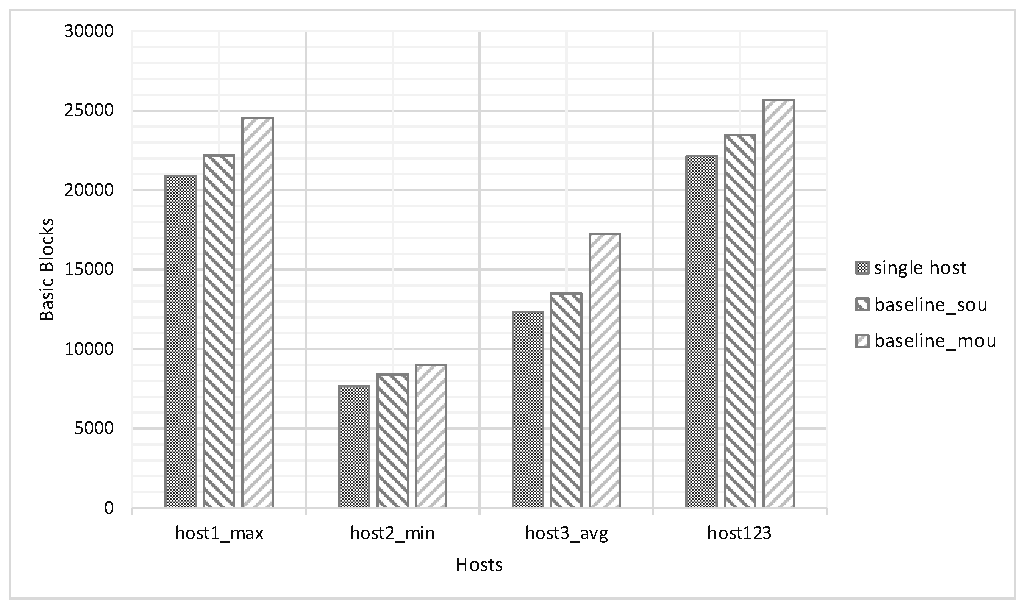
\includegraphics[width=\textwidth, clip=true,  trim= 0 0 0 0]{chapter5/ch5_baseline_code_coverage_crop.pdf}
 	\caption[پوشش کد برای هریک از میزبان‌ها و پوشش کدهای مبنا]
 	{
 		پوشش کد برای هریک از میزبان‌ها و پوشش کدهای مبنا.
 	}
 	\label{ch5_baseline_code_coverage_crop.pdf}
 	%\ref{ch5_baseline_code_coverage_crop.pdf}
 \end{figure}
 
 
 \subsubsection{مشاهدات}
 
 \begin{itemize}
 	\item{
 	میزان پوشش کد هریک از \lr{baseline}ها از پوشش کد فایل میزبان به تنهایی بیشتر است. یعنی تغییر میزبان‌ها منجر به اجرای بلوک‌های پایه جدید و احتمالاً مسیرهای اجرایی جدیدی، شده است.
 
}
\item {
میزان پوشش \lr{baseline}ها متناسب با میزبان‌ها است. یعنی به‌عنوان مثال \lr{host1\_max} بیشترین پوشش کد را در هر سه حالت تنها، \lr{baseline\_sou} و \lr{baseline\_mou} داشته است. این بدین معنی است که انتخاب فایل میزبان بسیار حائز اهمیت است و بخش قابل توجهی از پوشش کد در هر حالت مربوط به فایل میزبان است.

}

\item {
	میزان پوشش کد \lr{baseline\_mou} در تمامی میزبان‌ها از \lr{baseline\_sou} بیشتر است. این بدین معنی است که با افزایش میزان تغییر فایل شاهد افزایش میزان پوشش کد بوده‌ایم.
	
}

\item {
	 بیشترین پوشش کد مربوط به اجتماع پوشش کدهای \lr{baseline\_mou}  در \lr{host123} است که نشان می‌دهد هر کدام از میزبان‌ها مجموعه دستورات متفاوتی را اجرا کرده‌اند.
	
}

\item {
	درنهایت اعداد و ارقامِ پوشش کد در محدوده 25هزار بلوک پایه بوده که نشان می‌دهد \lr{MuPDF} نرم‌افزاری پیچیده است.
}

 \end{itemize}
 
 
 
 
 
 
\section{آزمایش‌ها، یافته‌ها و مقایسه نتایج} 
 در این بخش آزمایش‌های  صورت گرفته و نتایج حاصل از آن را بیان می‌کنیم. همچنین نتایج را با سایر کارهای مرتبط مقایسه خواهیم کرد. 
 چون \gls{SUT} مورد استفاده در یادگیری و فاز 
 \cite{Godefroid:2017:LML:3155562.3155573}
 برای آزمون دردسترس نبود، ما روش یادگیری و فاز را نیز پیاده‌سازی و آن را روی ابزار \lr{MuPDF} آزمایش کردیم. به‌این ترتیب توانستیم مقایسه معناداری بین روش پیشنهادی خود با این روش، به‌عنوان مرتبط‌ترین کار انجام شده داشته باشیم. نتایج نشان می‌دهد که روش پیشنهادی ما در معیار پوشش کد و همچنین در معیارهای خطا، دقت و سرگشتگی بهبود داشته است و توانسته روش یادگیری و فاز، که در آزمایش‌ها با نام \lr{laf} آن را نشان می‌دهیم، را شکست دهد. روش پیشنهادی ما همچنین نسبت به \lr{AFL} و \lr{AFL}افزوده بهبودهایی داشته است که خواهیم دید.
 
 چون مجموعه داده در مدل‌های یادگیری ژرف بسیار مهم است و روی نتایج تأثیر می‌گذارد در هنگام آموزش مدل \lr{laf} مجموعه داده را مطابق مقیاس ارائه شده در 
 \cite{Godefroid:2017:LML:3155562.3155573}
 لحاظ کردیم. بدین زمان آموزش کمتر برای هر دوره در حدود 15 دقیقه به طول انجامید. سایر پارامترها مانند طول توالی‌های آموزشی $d$ را که در مقاله به آن اشاره نشده بود نیز مشابه مقادیر آن در روش پیشنهادی قرار دادیم.
 
 
 \subsection{سرگشتگی، خطا و دقت مدل‌ها}
 
 جدول \ref{tabel:ppl_and_accuracy} سرگشتی، خطا و دقت مدل‌های چهارگانه پیشنهادی و مدل یادگیری و فاز را بعد از گذشت 50 دوره، روی مجموعه‌های آموزش و ارزیابی نشان می‌دهد. سرگشتی مطابق رابطه \ref{ppl} و خطا نیز از رابطه \ref{CrossEntropyLossFunction} برای مدل‌ها محاسبه شده است که در فصل \ref{chapter2} آنها را بیان کردیم. دقت نیز معیاری است که توسط \lr{Keras} برای هر مدل حساب می‌شود. همچنین  شکل \ref{ch5_loss_model2_vs_model_laf_crop.pdf} روند تغییرات خطا در فرایند آموزش را برای مدل 2 و مدل \lr{laf}  نشان می‌دهد. مدل 2 در این نمودار به‌این دلیل انتخاب گردیده که بیشترین میزان شباهت را از لحاظ معماری و مقادیر اَبرپارامترها با مدل \lr{laf} دارد. 
 
 
  \begin{table}%[ht]
 	\caption[سرگشتگی، دقت و خطای مدل‌های مختلف روی مجموعه‌های آموزش و ارزیابی]
 	{
 		سرگشتگی، دقت و خطای مدل‌های مختلف روی مجموعه‌های آموزش و ارزیابی.
 	}
 	\label{tabel:ppl_and_accuracy}
 	\centering
 	\onehalfspacing
 	\begin{tabularx}{0.95\linewidth}{r p{20mm} p{20mm} p{20mm} p{20mm} p{15mm}}
 		\toprule[1.5pt] 
 		معیار / مدل &
 		1 &
 		2 &
 		3 &
 		4 & 
 		\lr{laf}  
 		\\
 		\midrule[1.5pt] 
 		 سـرگــشتـگی &
 		$1.440$ &
 		$1.391$ &
 		$\boldsymbol{1.335}$ &
 		$1.350$ &
 		$1.860$
 		\\
 		%\hline 
 		بیشینه دقت آموزش &
 		$0.886$ &
 		$0.902$ &
 		$0.893$ &
 		$0.909$ &
 		$0.820$ 
 		\\
 		%\hline
 		بیشینه دقت ارزیابی &
 		$0.884$ &
 		$0.895$ &
 		$0.904$ &
 		$0.905$ &
 		$0.800$ 
 		\\
 		%\hline
 		کمینه خطای آموزش &
 		$0.353$ &
 		$0.298$ &
 		$0.324$ &
 		$0.276$ &
 		$0.623$ 
 		\\
 		%\hline
 		کمینه خطای ارزیابی &
 		$0.365$ &
 		$0.330$ &
 		$0.289$ &
 		$0.300$ &
 		$0.724$
 		\\
 		\bottomrule[1.5pt]
 		
 	\end{tabularx} 
 \end{table}
%\vspace{50mm}
 
  \begin{figure}%[ht]%[ht]%[tbh!]%%[t!]
 	\centering
 	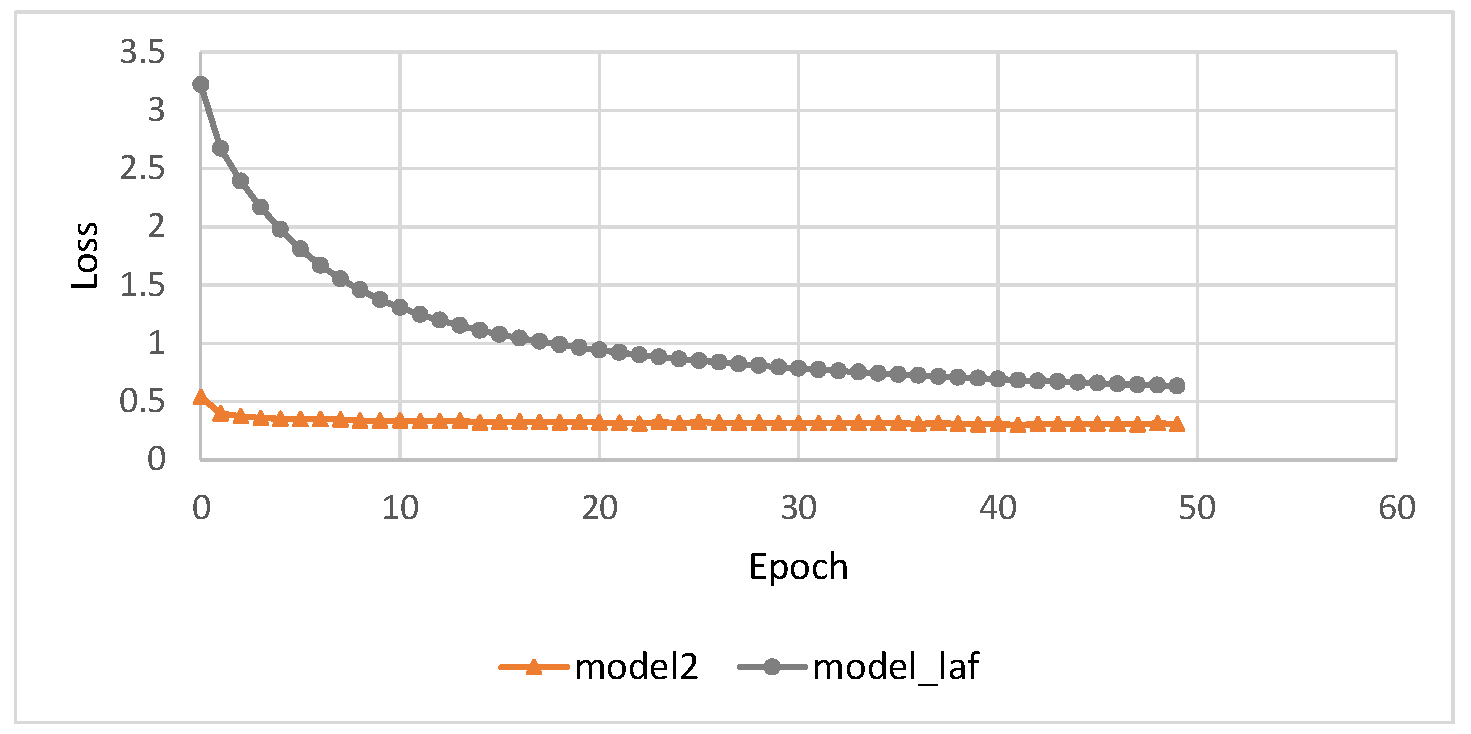
\includegraphics[width=\textwidth, clip=true,  trim= 0 0 0 0]{chapter5/ch5_loss_model2_vs_model_laf_crop.pdf}
 	\caption[نمودار تغییرات خطای مدل‌های 2 و \lr{laf}]
 	{
 	نمودار تغییرات خطای مدل‌های 2 و \lr{laf} در دوره‌های 1 تا 50.
 	}
 	\label{ch5_loss_model2_vs_model_laf_crop.pdf}
 	%\ref{ch5_loss_model2_vs_model_laf_crop.pdf}
 \end{figure}

\subsubsection{مشاهدات}

 \begin{itemize}
 	\item{
 سرگشتگی و خطای همه مدل‌های پیشنهادی از مدل یادگیری و فاز کمتر و دقت آنها از یادگیری و فاز بیشتر است. یعنی مدل زبانی عصبی با معماری توضیح داده شده در بخش \ref{sec:model}، در یادگیری ساختار فایل از مدل کدگذار-کدگشا 
 \cite{Godefroid:2017:LML:3155562.3155573}
 بهتر عمل کرده است.  	
 }
\item
{
	بیشترین دقت در بین تمامی مدل‌ها مربوط به مدل 4 است. مدل 4 \gls{LSTM} دوسویه است. شبکه \gls{LSTM} دوسویه هنگام آموزش علاوه‌بر کاراکترهای قبلی، کاراکترهای بعدی را نیز در نظر می‌گیرد. بنابراین توانسته‌ است بـه ‌دقت بیشتر دست یابد. کمترین میزان سرگشتگی نیز متعلق به مدل 3 است. این مدل همان‌طور که در جدول نیز مشخص است دارای کمترین خطای ارزیابی است. البته اختلاف بین مقادیر مختلف در همه مدل‌های پیشنهادی کم است که نشان می‌دهد همه مدل‌ها قادر به یادگیری و درک ساختار فایل بوده‌اند. 
	سرگشتگی بیشینه، حالت بدون استفاده از مدل یادگیری،  برای تنظیمات ما برابر 64 (اندازه بردار واژگان) خواهد بود.
}

\item
{
	در شکل \ref{ch5_loss_model2_vs_model_laf_crop.pdf}، منحنی خطای مدل 2 در همه دوره‌ها، از منحنی خطای مدل \lr{laf} پایین‌تر است. البته دوره‌ها زمان متفاوتی دارند بنابراین مقایسه نظیر‌به‌نظیر آنها ممکن است جالب به‌نظر نیاید. با این‌حال در بازه زمانی مساوی از شروع فرایند آموزش نیز این وضعیت فوق برقرار است. برای مثال پایان دوره‌ 1 برای مدل 2 مصادف با پایان دوره 12 برای مدل \lr{laf} خواهد بود که باز هم خطای مدل \lr{laf}  بیشتر است. ما فرایند آموزش را برای هر دو مدل تا دوره 100 ادامه دادیم و تغییر خلافی مشاهده نشد. چنان‌چه در بخش \ref{sec:epochcompare} خواهیم دید پوشش کد مدل 2 نیز در دوره‌های مختلف از مدل \lr{laf} بالاتر است.
}

 \end{itemize}
 
 \subsection{پوشش کد مدل‌های مولد}\label{sec:gen_model_cove}
 
 در آزمایش این بخش، مدل‌های مولد پیشنهادی  خود را برای اولین مرحله تولید داده آزمون محک می‌زنیم. برای تولید داده‌های آزمون جدید از روش نمونه‌برداری و پارامتر تنوع $D$ در همه آزمایش‌ها استفاده کردیم. همچنین هربار با یک پیشوند تصادفی از مجموعه آزمون تولید داده از مدل را شروع می‌کنیم. می‌خواهیم ببینیم برای میزبان‌های مختلف کدام مدل مولد و نیز کدام تنوع تولید داده، به پوشش کد بالاتری دست می‌یابد. هدف مقایسه کارکرد مدل‌ها و انتخاب مناسب‌ترین مدل برای استفاده در آزمون فازی است.
 برای این منظور هریک از مدل‌های جدول \ref{tabel:deep_model} را به تعداد 50 دوره آموزش دادیم. در پایان هر دوره یک نمونه از مدل آموزش دیده را ذخیره کردیم. سپس مدل با کمترین خطا را از بین نمونه‌های ذخیره شده، برای تولید داده برگزیدیم.
 
 
 در مرحله بعد برای هر مدل در هنگام تولید داده با هریک از تنوع‌های تولید $0.5$، $1$ و $1.5$، تعداد 1000 فایل \gls{PDF} با هر میزبان تولید کرده‌ایم. یعنی در مجموع با هر مدل و هر میزبان 3000 فایل را تولید می‌کنیم. چون 4 مدل و 3 میزبان داریم، درکل 36000 فایل تولید می‌شود و چون دو روش بروزرسانی شیء
  \gls{SOU} 
  و 
  \gls{MOU} هم نیاز است در نهایت 72000 فایل تولید می‌کنیم. دقت شود که در این مرحله هنوز عملیات آزمون فازی یعنی فاز ورودی، مشاهده رفتار برنامه در اشکال‌زدا و ذخیره خطاهای احتمالی، اعمال نشده است و تنها تأثیر مدل‌ها، تنوع تولید داده از آنها و میزبان‌ها، بر روی میزان پوشش کد مورد نظر است.
  
  \hspace{0.5mm}
  برای مقایسه با 
  \lr{baseline\_sou}
  تعداد 1000 شیء داده‌ای از هر مدل تولید کرده و برای مقایسه با 
  \lr{baseline\_mou}
  تعداد 3000 شیء داده‌ای با هر مدل تولید می‌کنیم. 
  تولید 1000 فایل
  \gls{PDF}
  جدید با استفاده از مدل‌ها برای حالت \gls{SOU}  (با اندازه بافر
  100\footnote{یعنی هر بار یک لیست از 100 شیء توسط مدل مولد بازگردانیده می‌شود.}) 
  به‌طور میانگین 60 دقیقه و برای حالت \gls{MOU} به‌طور میانگین 190 دقیقه به‌طول انجامید. در پایان پوشش کد نرم‌افزار \lr{MuPDF} روی هریک از 72 مجموعه 1000 فایلی اندازه‌گیری شد. ما همچنین ادغام پوشش‌های کد را برای هر تنوع در قالب \lr{host123} اندازه ‌گرفتیم. اندازه‌گیری پوشش کد برای هر مجموعه نیز در حدود 60 دقیقه زمان برد. کلیه نتایج به تفکیک میزبان‌ها در شکل‌های \ref{ch5_host1_max_crop} تا \ref{ch5_host123_crop.pdf}  ذکر شده است.
 
 
 
 \begin{figure}%[hbt]
	\centering
 	%\begin{longtable}{c}
 %% \lr{host1\_max}
 %\subfigure[برچسب 1]{%[ht]%[tbh!]%%[t!]
 \begin{subfigure}{\linewidth}
 	\centering
 	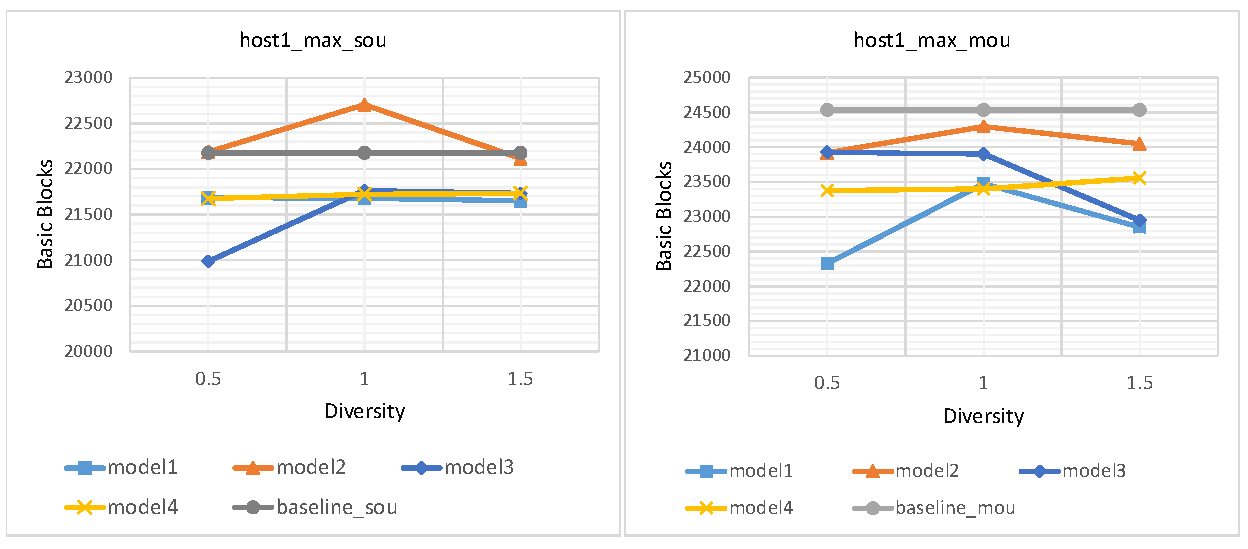
\includegraphics[width=\textwidth, clip=true,  trim= 0 0 0 0]{chapter5/ch5_host1_max_crop.pdf}
 	\caption[نمودار تغییرات پوشش کد در تنوع‌های نمونه‌برداری $0.5$ تا $1.5$  برای \_max\lr{host1}]
 	{
 		نمودار تغییرات پوشش کد در تنوع‌های نمونه‌برداری $0.5$ تا $1.5$  برای  \lr{host1\_max}.
 	}
 	\label{ch5_host1_max_crop}
 	%\ref{ch5_host1_max_crop}
 \end{subfigure}
	\vspace{0.75cm}

%% \lr{host2\_min}
  %\subfigure[برچسب 1]{%[ht]%[tbh!]%%[t!]
  \begin{subfigure}{\linewidth}

 	\centering
 	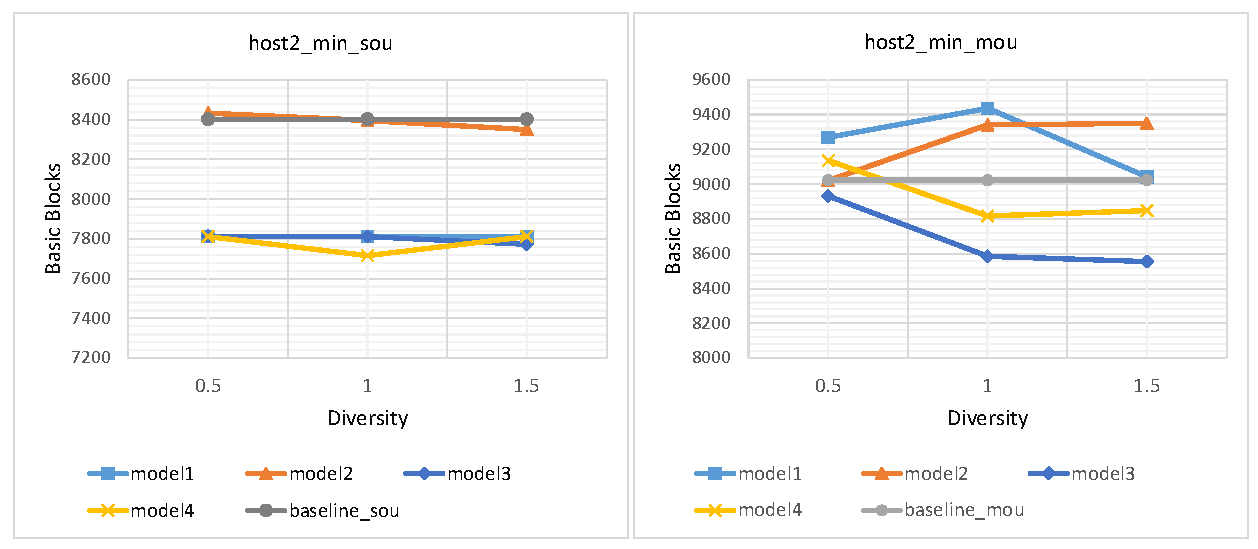
\includegraphics[width=\textwidth, clip=true,  trim= 0 0 0 0]{chapter5/ch5_host2_min_crop.pdf}
 	\caption[ تغییرات پوشش کد در تنوع‌های نمونه‌برداری $0.5$ تا $1.5$  برای  \lr{host2\_min}]
 	{
 		تغییرات پوشش کد در تنوع‌های نمونه‌برداری $0.5$ تا $1.5$  برای \lr{host2\_min}.
 	}
 	\label{ch5_host2_min_crop.pdf}
 	%\ref{ch5_host2_min_crop.pdf}
\end{subfigure}
\vspace{1cm}

 \caption[نمودار تغییرات پوشش کد مدل‌های مختلف برحسب تنوع.]{
 	 نمودار تغییرات پوشش کد مدل‌های مختلف برحسب تنوع.   
  }
 
\end{figure}


 \begin{figure}%[hbt]
 	\ContinuedFloat
 
%% \lr{host3\_avg}
%\subfigure[برچسب 1]{%[ht]%[tbh!]%%[t!]
 \begin{subfigure}{\linewidth}
	\centering
	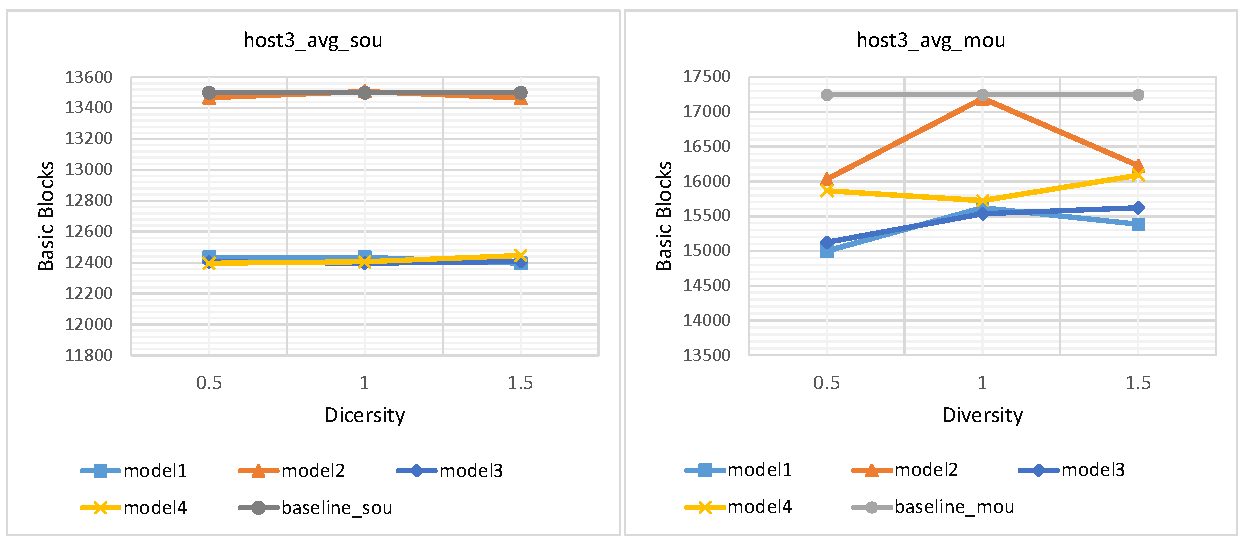
\includegraphics[width=\textwidth, clip=true,  trim= 0 0 0 0]{chapter5/ch5_host3_avg_crop.pdf}
	\caption[ تغییرات پوشش کد در تنوع‌های نمونه‌برداری $0.5$ تا $1.5$  برای  \lr{host3\_avg}]
	{
		تغییرات پوشش کد در تنوع‌های نمونه‌برداری $0.5$ تا $1.5$  برای \lr{host3\_avg}.
	}
	\label{ch5_host3_avg_crop.pdf}
	%\ref{ch5_host3_avg_crop.pdf}
	
\end{subfigure}
 \vspace{0.75cm}
 
 %% \lr{host123}
 %\subfigure[برچسب 4]{%[ht]%[tbh!]%%[t!]
 \begin{subfigure}{\linewidth}
 	\centering
 	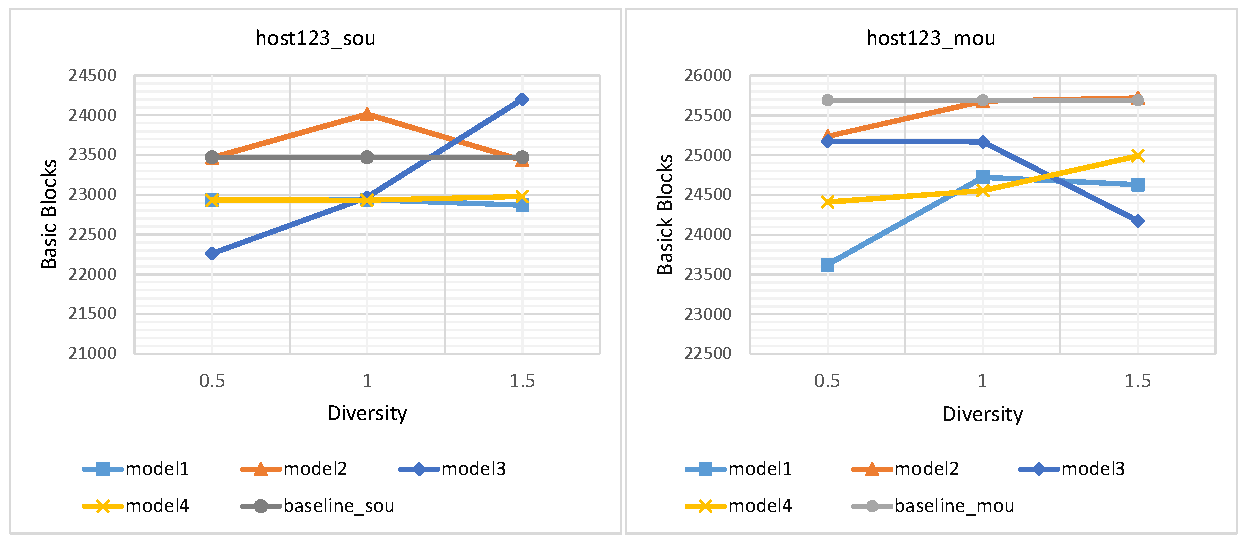
\includegraphics[width=\textwidth, clip=true,  trim= 0 0 0 0]{chapter5/ch5_host123_crop.pdf}
 	\caption[تغییرات پوشش کد در تنوع‌های نمونه‌برداری $0.5$ تا $1.5$  برای  \lr{host123}]
 	{
 	تغییرات پوشش کد در تنوع‌های نمونه‌برداری $0.5$ تا $1.5$  برای \lr{host123}.
 	}
 	\label{ch5_host123_crop.pdf}
 	%\ref{ch5_host123_crop.pdf}

\end{subfigure}
\vspace{1cm}
%\end{longtable}

\caption[]{(ادامه.)
	نمودار تغییرات پوشش کد مدل‌های مختلف برحسب تنوع.    
}

 \end{figure}




 \subsubsection{مشاهدات}
 \begin{itemize}
 	\item {
 	پوشش کد داده‌های تولیدی از پوشش کد مبنا در اکثر موارد کمتر است؛ زیرا، اشیای تولید شده به خوش‌شکلی اشیای واقعی نیستند. البته دربرخی موارد شاهد افزایش پوشش کد هستیم. از جمله برای  \lr{host2\_min}
 در حالت \gls{MOU}.
}
\item{
تولید داده با تنوع 1 در بیشتر مدل‌ها و روی اکثریت میزبان‌ها پوشش کد بهتری داشته است. یعنی پارامتر تنوع واقعاً سبب بدشکل شدن و بالا رفتن گوناگونی داده‌های تولید شده و در نتیجه پارامــتری مؤثر بوده است.
	
}

\item{
	
	افزایش تنوع در مدل \gls{LSTM} دوسویه در حالت کلی سبب افزایش پوشش کد شده است؛ اما در دیگر مدل‌ها خیر.

}

\item{
تقریباً در همه نمودارها داده‌های تولید شده توسط مدل 2، پوشش کد بیشینه را نتیجه داده است. یعنی مدل‌های ژرف ساده بهتر از مدل‌های ژرف پیچیده همچون \lr{LSTM} دوسویه (مدل 4)، عمل کرده‌اند. به‌همین دلیل مدل 2 با تنوع تولید داده 1 پیروز نهایی این سری از آزمایش‌های ما هستند.

}

 \end{itemize}


\subsection{مقایسه با مدل کدگذار-کدگشا}

برای مقایسه با 
\cite{Godefroid:2017:LML:3155562.3155573}
ابتدا مدل کدگذار-گشای توضیح داده شده را پیاده‌سازی و آن 50 دوره آموزش دادیم. سپس 1000 فایل \lr{PDF} را با این مدل تولید و پوشش کد مجموع آنها را انداز‌ه‌گیری کردیم. چون راهبرد نمونه‌برداری برای مدل مذکور نیز بهترین روش گزارش شده است، ما نیز از نمونه‌برداری برای تولید داده‌ها با این مدل استفاده کرده‌ایم. برای مدل‌های چهارگانه خود نیز بالاترین پوشش کد کسب شده در میان همه تنوع‌های آزمایش شده در بخش \ref{sec:gen_model_cove} را به‌عنوان  نماینده پوشش کد برای هر مدل انتخاب کردیم. در نهایت  دو حالت \gls{SOU} و \gls{MOU} را به‌صورت مجزا مورد ارزیابی و مقایسه قرار دادیم. نتایج در شکل \ref{ch5_cmp_laf} نشان داده شده است. شکل \ref{ch5_cmp_laf_sou_crop.pdf} حالت \gls{SOU} و شکل  \ref{ch5_cmp_laf_mou_crop.pdf} حالت \gls{MOU} را نشان می‌دهد.

 
 \begin{figure}%[hbt]
 	\centering
 	%% SOU
	\begin{subfigure}{\linewidth}
		
		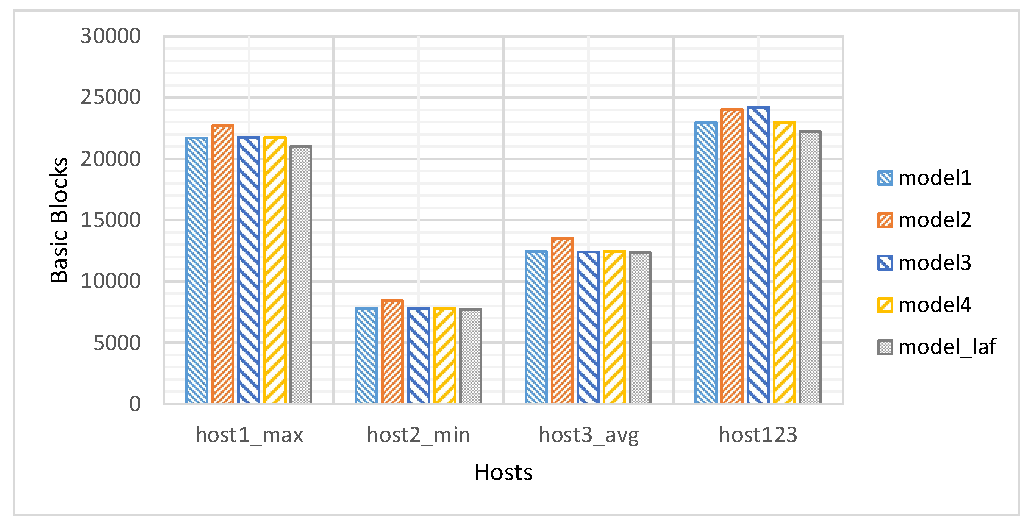
\includegraphics[width=\textwidth, clip=true,  trim= 0 0 0 0]{chapter5/ch5_cmp_laf_sou_crop.pdf}
		\caption
		{
			حالت \gls{SOU}.
		}
		\label{ch5_cmp_laf_sou_crop.pdf}
		%\ref{ch5_cmp_laf_sou_crop.pdf}
		
	\end{subfigure}
	\vspace{0.75cm}
	
	%% MOU
	\begin{subfigure}{\linewidth}
		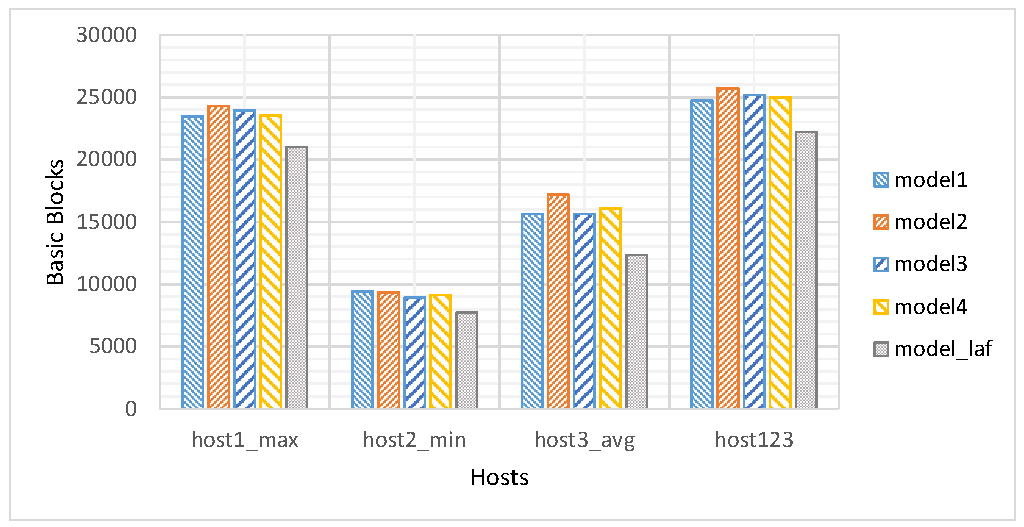
\includegraphics[width=\textwidth, clip=true,  trim= 0 0 0 0]{chapter5/ch5_cmp_laf_mou_crop.pdf}
		\caption
		{
			حالت \gls{MOU}.
		}
		\label{ch5_cmp_laf_mou_crop.pdf}
		%\ref{ch5_cmp_laf_mou_crop.pdf}
		
	\end{subfigure}
	\vspace{1cm}
	%\end{longtable}
	
	\caption[]{
		    نمودار پوشش کد‌ مدل‌های مختلف در مقایسه با مدل \lr{laf} برحسب فایل‌های میزبان‌.
	    
    }
	\label{ch5_cmp_laf}
\end{figure}%


\subsubsection{مشاهدات}
\begin{itemize}
	\item{
در حالت \gls{SOU} و برای \lr{host1\_max} همه مدل‌های پیشنهادی پوشش کد بالاتری داشته‌اند. در همین حالت دو میزبان دیگر اختلاف پوشش کد ناچیز بوده است. اما در حالت اجتماع پوشش کدها یعنی \lr{host123} مدل‌های پیشنهادی بهتر ظاهر شده‌اند یعنی هر مدل برای هر میزبان مجموعه دستورات متفاوتی را اجرا کرده است.
}

	\item{
	در حالت \gls{MOU} مدل‌های پیشنهادی ما با اختلاف بهتر هستند. این نشان می‌دهد که تغییر بیشتر فایل‌های میزبان به افزایش پوشش کد، در تعداد داده آزمون مساوی، می‌انجامد. بنابراین حالت \gls{MOU} را برای انجام آزمون فازی توصیه می‌کنیم. 
}
\item{
	در هر دو حالت اختلاف بین پوشش کد مدل‌ها برای \lr{host2\_min} کمتر و برای \lr{host1\_max} بیشتر به‌چشم می‌خورد. این امر نشان می‌دهد که انتخاب فایل میزبان در مواردی که نیاز به آن هست، مانند فایل \gls{PDF} که ساختار پیچیده‌ای دارد و یادگیری کامل آن به‌آسانی محقق نمی‌شود، بسیار حائز اهمیت است و تأثیر چشم‌گیری روی ارتقاء پوشش کد دارد. این انتخاب نبایست تصادفی انجام شود، چون دیدیم افزایش پوشش کد رابطه مستقیمی با پوشش کد فایل میزبان دارد. بنابراین فایل میزبان با پوشش کد بیشتر را برای انجام آزمون فازی توضیه می‌کنیم.
	
}

\end{itemize}


\subsection{مقایسه در دوره‌های مختلف}\label{sec:epochcompare}

یک پارامتر قابل ارزیابی که در جدول \ref{tabel:all_parameters} مطرح کردیم و تأثیر آن روی پوشش کد در 
\cite{Godefroid:2017:LML:3155562.3155573}
نیز بررسی شده است تعداد دوره‌های آموزش است. به نظر می‌رسد که پوشش کد ارتباط مستقیمی با تعداد دوره‌های آموزش مدل ژرف داشته باشد. برای این منظور پوشش کد 1000 فایل تولید شده با استفاده از مدل 2 را در سه دوره $10$، $30$ و $50$ اندازه‌گیری کردیم. سپس همین کار را برای مدل \lr{laf} نیز انجام دادیم. برای آن که نتایج قابل اطمینان باشند و اثر پارامترهای تصادفی از بین برود، هر آزمایش را سه مرتبه با سه مجموعه داده مجزا تکرار و میانگین پوشش کدها اندازه گرفتیم. نتایج در شکل \ref{ch5_cmp_epochs_crop.pdf} نشان داده شده‌اند.



 \begin{figure}%[ht]%[ht]%[tbh!]%%[t!]
	\centering
	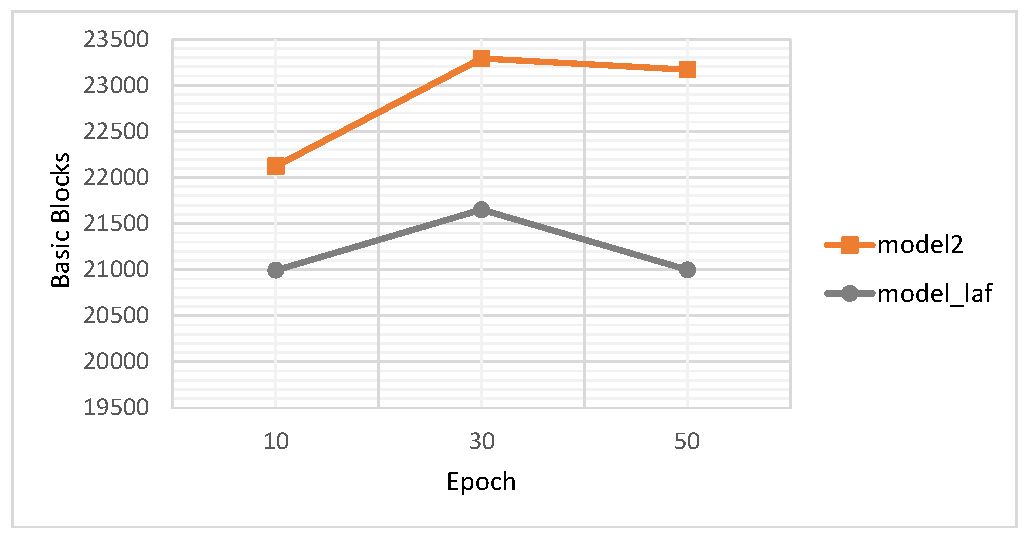
\includegraphics[width=\textwidth, clip=true,  trim= 0 0 0 0]{chapter5/ch5_cmp_epochs_crop.pdf}
	\caption
	{
		نمودار تغییرات پوشش کد برحسب دوره برای مدل‌های 2 و \lr{laf}.
	}
	\label{ch5_cmp_epochs_crop.pdf}
	%\ref{ch5_cmp_epochs_crop.pdf}
\end{figure}

\subsubsection{مشاهدات}
\begin{itemize}
	\item{
برای هر دو مدل پوشش کد از دوره 10 به 30 افزایش و سپس در دوره 50 کاهش یافته است. یعنی رابطه مستقیم معناداری بین پوشش کد و تعداد دوره‌های آموزش مدل وجود ندارد. 	

}
\item{
با بررسی مقدار خطای مدل در هر دوره متوجه شدیم تا زمانی که نرخ کاهش خطای مدل در فرایند آموزش زیاد است، پوشش کد نیز افزایش می‌یابد؛ چراکه ساختار فایل بهتر یادگیری شده و در نتیجه مدل قادر به تولید داده‌های خوش‌شکل‌تری خواهد بود. هنگامی که نرخ کاهش خطا از یک حد آستانه کمتر می‌شود، افزایش پوشش کد نیز ثابت شده یا اندکی کاهش می‌یابد. 
}

\item{
	در همه دوره‌های شکل \ref{ch5_cmp_epochs_crop.pdf} پوشش کد مدل پیشنهادی از مدل \lr{laf} بیش‌تر بوده است که نشان می‌دهد این مدل ساختار فایل را بهتر یادگرفته است. 
}
	
\end{itemize}

\subsection{آزمون فازی عصبی}
در پنجمین و آخرین آزمایش نرم‌افزار \lr{MuPDF} را با استفاده از فازر پیشنهادی در بخش \ref{ch4_iust_deep_fuzzer_crop.pdf}، مورد آزمون فازی قرار دادیم. برای این منظور الگوریتم‌های فاز عصبی داده و فاز عصبی فراداده (الگوریتم‌های \ref{alg:data_neural_fuzz} و \ref{alg:metadata_neural_fuzz}) را که در بخش \ref{sec:neural_fuzzing_algorithms} معرفی کرده بودیم، پیاده‌سازی و با استفاده از هریک از آنها تعداد $10000$ فایل \gls{PDF} را ایجاد کردیم. تنظیمات پارامترهای ورودی و ثوابت موجود در الگوریتم‌های پیشنهادی به قرار جدول 
\ref{table:alg-inputs}
 است. ستون آخر جدول
\ref{table:alg-inputs}،
همچنین مقادیر مجاز برای هریک از ورودی‌ها و ثوابت داده شده را نشان می‌دهد. حداکثر طول یک شیء داده‌ای 
\lr{PDF}
را در بازه متغیر 450 تا 550 انتخاب کرده‌ایم؛ زیرا، به طور میانگین طول اشیای استخراج شده مجموعه‌های آموزش و آزمون، در این بازه قرار دارد.
در آزمایش‌های آتی خود در نظر داریم تا آزمون فازی را با مقادیر متنوع انتخابی از مجموعه‌های داده شده انجام دهیم و بدین ترتیب قادر خواهیم بود تا اثر هریک از این پارامترها را به طور دقیق‌تری بررسی کنیم.


ما همچنین نسخه‌هایی از الگوریتم‌های \ref{alg:random_fuzz} 
\cite{Sutton:2007:FBF:1324770}
و \ref{alg:sample_fuzz} 
\cite{Godefroid:2017:LML:3155562.3155573}
را پیاده‌سازی و آزمون فازی را با تولید داده آزمون از طریق این الگوریتم‌ها نیز انجام دادیم. برای حالت تصادفی (الگوریتم \ref{alg:random_fuzz}) از ابزار \lr{FileFuzz} که یک فازر تصادفی تحت سیستم عامل ویندوز است و در بخش \ref{sec:fuzzer} معرفی شد، استفاده کردیم. متأسفانه در روش یادگیری و فاز 
\cite{Godefroid:2017:LML:3155562.3155573}،
تقریباً اکثر ابرپارامترهای مورد نیاز در هنگام آزمایش‌ها نامشخص هستند و نویسندگان اشاره‌ای به مقادیر آنها نکرده‌اند. برای این هریک از این ابرپارامترها نظیر 
$d$،
ما همان مقدار استفاده شده در الگوریتم‌های روش ‌پیشنهادی را استفاده کردیم، تا بدین ترتیب شرایط یکسانی بر آزمایش‌ها حاصل باشد. در همه آزمایش‌ها، \lr{host1\_max} به‌عنوان میزبان\footnote{در تولید داده آزمون به روش تصادفی و روش مبتنی برجابه‌جایی، به‌جای میزبان، به یک یا تعدادی دانه اولیه نیاز داریم که در اینجا از همان  \lr{host1\_max} استفاده گردید.}
 استفاده شد. نتایج حاصــل از پوشش کد روش‌های مختلف در جدول \ref{tabel:neural_fuzzing_result} آمده است. همچنین جدول \ref{tabel:neural_fuzzing_result_compare} میزان بهبود در پوشش کد روش پیشنهادی در مقایسه با کارهای مرتبط را نشان می‌دهد. 



\begin{table}
	\caption{مقادیر مجاز و مقادیر داده شده به ثوابت و ورودی‌های الگوریتم‌های فازی عصبی داده و فاز عصبی فرا داده در هنگام آزمون فازی قالب فایل \lr{PDF} }
	\centering
	\label{table:alg-inputs}
	\begin{tabular}{@{}rrr@{}}
		\toprule[1.5pt]
		\multicolumn{1}{r}{پارامتر ورودی / ثابت}                           & \multicolumn{1}{r}{مقادیر استفاده شده} & \multicolumn{1}{r}{مقادیر مجاز}                      \\ \midrule[1.5pt]
		\begin{tabular}[c]{@{}r@{}}\lr{Learnt model M}\end{tabular}  & 2    & \begin{tabular}[c]{@{}r@{}}$1,2,3,4, laf$\end{tabular}    \\
		\begin{tabular}[c]{@{}r@{}}\lr{Sequence prefix P}\end{tabular}      & انتخاب از مجموعه آزمون          & \begin{tabular}[c]{@{}l@{}} ثابت رشته‌ای\end{tabular} \\
		\begin{tabular}[c]{@{}r@{}}\lr{Diversity D}\end{tabular}            & 1                               & \begin{tabular}[c]{@{}r@{}}$(0, +\infty)$\end{tabular}           \\
		\begin{tabular}[c]{@{}r@{}}\lr{Fuzzing rate FR}\end{tabular}        & $0.10$                             & \begin{tabular}[c]{@{}r@{}}$(0,1]$\end{tabular}        \\
		\begin{tabular}[c]{@{}r@{}}\lr{End token ET}\end{tabular}           & \lr{endobj}                          & \begin{tabular}[c]{@{}r@{}}ثابت رشته‌ای\end{tabular} \\
		\begin{tabular}[c]{@{}r@{}}\lr{Binary token BT}\end{tabular}        & stream                          & \begin{tabular}[c]{@{}l@{}}ثابت رشته‌ای\end{tabular} \\
		$(a,b)$                                                              & $(450,550)$                       & \begin{tabular}[c]{@{}r@{}}$(len(P), +\infty)$\end{tabular}    \\
		\begin{tabular}[c]{@{}r@{}}$\alpha$   (\lr{DataNeuralFuzz})\end{tabular}     & $0.50$                            & \begin{tabular}[c]{@{}l@{}}$(0,1)$\end{tabular}          \\
		\begin{tabular}[c]{@{}l@{}}$\beta$   (\lr{MetadataNeuralFuzz})\end{tabular} & $0.90$ & \begin{tabular}[c]{@{}l@{}}$(0,1)$\end{tabular}          \\ \bottomrule[1.5pt]
	\end{tabular}
\end{table}



\begin{table}%[ht]
	\caption[نتایج پوشش کد حاصل از آزمون فازی نرم‌افزار \lr{MuPDF} با الگوریتم‌های تولید داده آزمون مختلف]
	{
		نتایج پوشش کد حاصل از آزمون فازی نرم‌افزار \lr{MuPDF} با الگوریتم‌های تولید داده آزمون مختلف.‌
	}
	\label{tabel:neural_fuzzing_result}
	\centering
	\onehalfspacing
	\begin{tabularx}{1.0\linewidth}{r r r r r}
		\toprule[1.5pt] 
		الگوریتم تولید داده آزمون / معیار &
		 پوشش بلوک پایه &
		 درصد \hspace{15mm} &
		 پوشش خط‌کد &
		 درصد
		\\
		\midrule[1.5pt] 
		\lr{DataNeuralFuzz} &
		$23719$ &
		$19.36$ &
		$18673$ &
		$20.81$
		\\
		%\hline 
		\lr{MetadataNeuralFuzz} &
		$22583$ &
		$18.43$ &
		$17894$ &
		$19.95$
		\\
		%\hline 
		\lr{SampleFuzz} \cite{Godefroid:2017:LML:3155562.3155573} &
		$20957$ &
		$17.10$ &
		$16793$ &
		$18.72$
		\\
		%\hline 
		\lr{RandomFuzz (FileFuzz)} \cite{Sutton:2007:FBF:1324770} &
		$7563$ &
		$6.17$ &
		$5002$ &
		$5.58$
		\\
		\bottomrule[1.5pt]
		
	\end{tabularx} 
\end{table}




\begin{comment}


\begin{table}%[ht]
	\caption[میزان بهبود پوشش کد ابزار  \lr{MuPDF}توسط الگوریتم‌های روش پیشنهادی در مقایسه با کارهای مرتبط.]
	{
		میزان بهبود پوشش کد ابزار \lr{MuPDF} توسط الگوریتم‌های روش پیشنهادی در مقایسه با کارهای مرتبط. اعداد داخل جدول به‌صورت درصد هستند. مقادیر هر خانه برابر اختلاف پوشش کد حاصله از الگوریتم‌های ستون و سطر مربوط به آن مقدار است.
	}
	\label{tabel:neural_fuzzing_result_compare2}
	\centering
	\onehalfspacing
	\begin{tabularx}{0.95\linewidth}{r p{35mm} p{35mm}}
		\toprule[1.5pt] 
		الگوریتم تولید داده آزمون &
		\lr{DataNeuralFuzz} &
		\lr{MetadataNeuralFuzz}
		\\
		\midrule[1.5pt] 
	    \lr{SampleFuzz} \cite{Godefroid:2017:LML:3155562.3155573} &
		$+2.26$ &
		$+1.83$
		\\
		%\hline 
		\lr{AFL} \cite{DBLP:journals/corr/abs-1711-04596} &
		$+7.73$ &
		$+6.80$
		\\
		%\hline 
		\lr{Augmented AFL } \cite{DBLP:journals/corr/abs-1711-04596} &
		$+7.56$ &
		$+6.63$	
		\\
		%\hline 
		\lr{RandomFuzz (FileFuzz)} \cite{Sutton:2007:FBF:1324770} &
		$+13.19$ &
		$+12.26$
		\\
		\bottomrule[1.5pt]
		
	\end{tabularx} 
\end{table}
\end{comment}

%\vspace{1cm}

\begin{table}
	\caption[میزان بهبود پوشش کد ابزار  \lr{MuPDF}توسط الگوریتم‌های روش پیشنهادی در مقایسه با کارهای مرتبط.]
	{
		میزان بهبود پوشش کد ابزار \lr{MuPDF} توسط الگوریتم‌های روش پیشنهادی در مقایسه با کارهای مرتبط. اعداد داخل جدول به‌صورت درصد هستند. مقادیر هر خانه برابر اختلاف پوشش کد حاصله از الگوریتم‌های ستون و سطر مربوط به آن مقدار است.
	}
	\label{tabel:neural_fuzzing_result_compare}
	\centering
	\onehalfspacing
	\begin{tabular}{@{}rrr@{}}
		\cmidrule[1.5pt](l){2-3}
		& \multicolumn{2}{c}{روش پیشنهادی}                                                                               \\ \midrule[1.5pt]
		\multicolumn{1}{r}{روش‌های موجود}           & \multicolumn{1}{r}{\lr{DataNeuralFuzz}} & \multicolumn{1}{r}{\lr{MetaDataNeuralFuzz}} \\ \midrule
		\lr{SampleFuzz} \cite{Godefroid:2017:LML:3155562.3155573}            & $+2.26$                                                  & $+1.83$                                                      \\
		\lr{AFL} \cite{DBLP:journals/corr/abs-1711-04596}                  & $+7.73$                                                  & $+6.80$                                                      \\
		\lr{AugmentedAFL} \cite{DBLP:journals/corr/abs-1711-04596}         & $+7.56$                                                  & $+6.63$                                                      \\
		\lr{RandomFuzz (FileFuzz)} \cite{Sutton:2007:FBF:1324770}& $+13.19$                                                 & $+12.26$                                                     \\ \bottomrule[1.5pt]
	\end{tabular}
\end{table}




\subsubsection{مشاهدات}

\begin{itemize}
	\item{
الگوریتم فاز عصبی فراداده به پوشش کد کمتری دست پیدا کرده است، زیرا همان‌طور که انتظار می‌رود دستکاری بخش کوچکی در از قالب فایل ممکن است آن را کاملاً نامعتبر کند و در مرحله اولیه تجزیه توسط تجزیه‌گر رد شود. بنابراین الگوریتم در رسیدن به هدف خود یعنی فاز فراداده موفق بوده است.  	
}
\item{
هر دو الگوریتم فاز عصبی داده و فاز عصبی فراداده پوشش کد بهتری نسبت به
\lr{SampleFuzz}
داشته‌اند که نشان از عملکرد بهتر مد‌ل‌های پیشنهادی در یادگیری ساختار فایل و عملکرد بهتر الگوریتم‌های پیشنهادی در فاز کردن این فایل‌ها دارد. پوشش کد حاصل شده در این آزمایش‌ها همچنین از پوشش کد گزارش شده در 
\cite{DBLP:journals/corr/abs-1711-04596}
که حاصل از آزمون فازی \lr{MuPDF} با  \lr{AFL} و \lr{AFL} افزوده بیشتر است. اعداد مربوط به آنها قبلاً در بخش \ref{sec:augmented_afl_problems} ذکر شدند. جدول \ref{tabel:neural_fuzzing_result_compare} در این بخش نیز اختلاف این مقادیر را با مقادیر حاصل از پوشش کد روش پیشنهادی نشان داده است.
	 
}
\item{
به‌وضوح می‌توان برتری روش‌های هوشمند تولید داده آزمون را نسبت به روش‌های تصادفی مشاهده کرد. همانطور که در ابتدای این پایان‌نامه گفتیم روش‌های تصادفی در ساختارهای پیچیده پوشش کد بسیار کمی را نتیجه می‌دهند. پوشش کد الگوریتم فاز عصبی داده بیش از 3 برابر الگوریتم فاز تصادفی است.
}

\item{
باوجود استفاده از هوش‌مصنوعی و الگوریتم‌های هوشمند در تولید داده آزمون همچنان شاهد پوشش کد پایینی (کمتر از 20 درصد) در پایان عملیات آزمون هستیم. به‌نظر می‌رسد رسیدن به پوشش کد بالا در ساختارهای پیچیده، با آزمون فازی جعبه سیاه کار دشواری باشد. از طرفی فنون آزمون جعبه سفید مانند روش‌های اجرای نمادین نیز روی این ساختارها به‌علت پیچیدگی بالا و وجود محدودیت‌های فراوان سخت، زمان‌بر و تا حد زیادی غیرممکن است و کماکان آزمون فازی مؤثرتر بوده است.   
}
\end{itemize}



\subsubsection{خطا‌ها و آسیب‌پذیری‌های شناسایی شده}
در بررسی گزارش‌های تولید شده توسط \lr{Application Verifier} پس از هر آزمون، هیچ‌گونه خطایی مشاهده نکردیم. باتوجه به‌اینکه ما نسخه نهایی نرم‌افزار \lr{MuPDF} را مورد آزمایش قرار دادیم، تصور می‌شود که بیشتر خطا‌های آن در نسخه‌های آزمایشی برطرف شده باشد و در نتیجه پیدا کردن خطای جدید سخت خواهد بود. از طرفی \lr{MuPDF} نرم‌افزاری تحت توسعه فعال و جامعه توسعه‌دهنده و کاربری بزرگی است که سبب می‌شود تا از کیفیت خوبی برخوردار باشد. با این حال الگوریتم فاز عصبی داده چندین مورد استفاده از توابع ناامن را شناسایی کرد که \lr{Application Verifier} آنها را درقالب هشدارهای امنیتی اعلام کرده است. 

پیش از آزمایش‌های اصلی ما فازر و \lr{Application Verifier} روی نرم‌افزارهای کوچکی که خطای آنها مشخص بود اجرا کردیم. به‌نظر می‌رسد \lr{Application Verifier} روی ویندوز 10 نسخه 64 بیتی قادر به تشخیص خطاهای حافظه برنامه‌های 32 بیتی نیست؛ زیرا موفق به شناسایی این خطاها نشدیم. برای برنامه‌های 64 بیتی اما این مشکل وجود نداشت. لذا ما هر دو نسخه 32 و 64 بیتی \lr{MuPDF} را مورد آزمون قرار دادیم. 

فازر، برنامه \lr{PDF}خوان را با داده آزمون ورودی باز و بعد از 10 ثانیه آن را بسته و برای تزریق داده آزمون بعدی اقدام می‌کند. همزمان پوشش کد و گزارش وضعیت حافظه نیز ثبت و ذخیره می‌شوند. بنابراین زمان آزمون برای هر مجموعه 10000 فایلی حدود 28 ساعت به‌طول انجامید\footnote{\lr{Application Verifier}
		 و ابزارگذاری کد سربارهایی را به زمان هربار اجرای برنامه اضافه می‌کنند. همچنین فاصله زمانی کوتاهی بین تزریق داده‌های آزمون متوالی درنظر گرفته شد؛ زیرا، در مواردی سقوط برنامه ناشی از خطای دیگر بخش‌های سیستم است. با لحاظ این زمان‌ها از سقوط‌های این چنینی با اطمینان زیادی جلوگیری می‌نماییم.
	  }. 
برای همه نرم‌افزارهای دیگر آزمون به‌این شیوه قابل انجام خواهد بود. گفتیم که آزمون فازی نوعی آزمون فشار است. در نظر داریم تا آزمون فازی با این روش را با استفاده از $100$ هزار فایل تولید شده و حتی بیشتر انجام دهیم. در این صورت امکان سقوط برنامه \lr{MuPDF} افزایش می‌یابد.



\subsubsection{تنوع داده‌های تولید شده}
مدل‌های ما در روش پیشنهادی قادر به تولید داده‌های متنوع و به‌صورت کنترل شده بدشکل هستند. الگوریتم فاز عصبی داده به‌خوبی در تغییر محتویات فایل‌های 
\lr{PDF}
عمل کرده و می‌تواند فایل‌هایی با داده‌های جدید بدون تغییر در ساختار ایجاد کند. شکل \ref{ch5_amazing_generated_test_data.png} نمونه‌ای از داده‌های تولید شده توسط الگوریتم فاز عصبی داده را نشان می‌دهد. همان‌طورکه در این شکل پیداست فایل‌های \lr{PDF} در عین معتبر بودن حاوی داده‌های جدیدی هستند که با مقادیر مرزی در فرایند تولید داده آزمون جایگذاری شده‌اند. به‌دلیل معتبر بودن تعداد بیشتری از فایل‌های تولید شده توسط الگوریتم فاز عصبی داده پوشش کد این الگوریتم از پوشش کد الگوریتم فاز عصبی فراداده بیشتر است. اما هر دو الگوریتم مورد نیاز هستند؛ زیرا، هرکدام مرحله مجزایی از مراحل پردازش فایل در کد برنامه را هدف آزمون قرار می‌دهند.



\begin{figure}[ht]%[ht]%[tbh!]%%[t!]
	\centering
	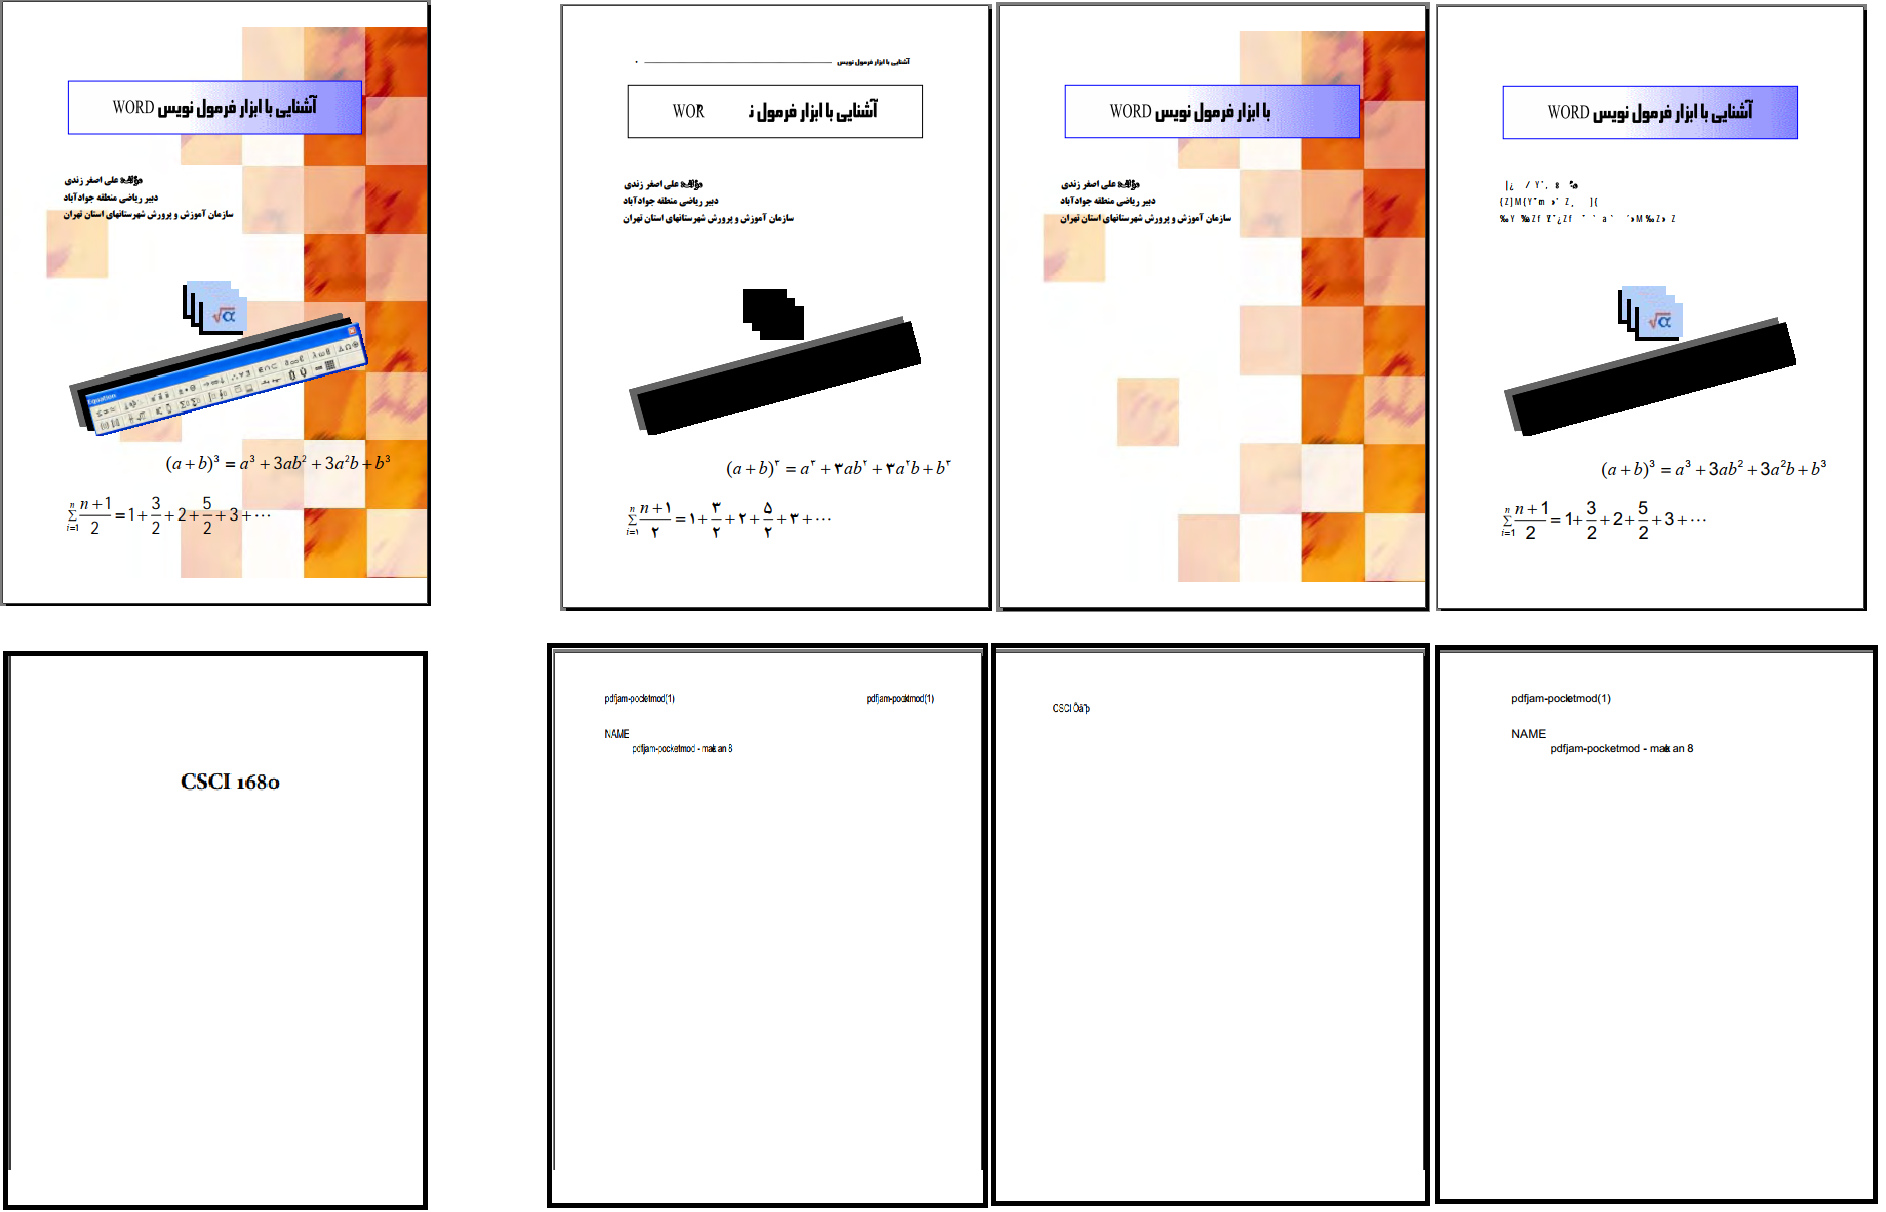
\includegraphics[width=0.95\textwidth, clip=true,  trim= 0 0 0 0]{chapter5/ch5_amazing_generated_test_data.png}
	\caption[نمونه‌ای از داده‌های آزمون متنوع تولید شده توسط الگوریتم فاز عصبی داده در فرایند آزمون فازی قالب فایل \lr{PDF}.]
	{
		نمونه‌ای از داده‌های آزمون متنوع تولید شده توسط الگوریتم فاز عصبی داده در فرایند آزمون فازی قالب فایل \lr{PDF}. در هر ردیف، سمت چپ‌ترین فایل، فایل میزبان را نشان می‌دهد و 3 فایل سمت راست فایل‌های حاصل از مدل مولد هستند. تغییر در محتوا به وضوح قابل مشاهده است.
	}
	\label{ch5_amazing_generated_test_data.png}
	%\ref{ch5_cmp_epochs_crop.pdf}
\end{figure}





\section{خلاصه}
در این فصل، ابتدا پارامترهای قابل بررسی و مؤثر در روش‌های تولید داده آزمون مبتنی بر یادگیری ژرف را معرفی و سپس روش پیشنهادی خود را که در فصل \ref{ch:4} مطرح کرده بودیم، روی نرم‌افزار \lr{MuPDF} و برای مهمترین این پارامترها مورد آزمایش و ارزیابی قرار دادیم. نتایج در حالت کلی حاکی از بهبود میزان پوشش کد در آزمون فازی \lr{MuPDF} هنگام استفاده از مدل‌های و الگوریتم‌های تولید داده آزمون پیشنهاد شده است. به‌خصوص نسبت به تعدادی از روش‌های قبلی از جمله 
\cite{Godefroid:2017:LML:3155562.3155573}
که مشابه‌ترین کار مرتبط بود، آمار و ارقام بهتری هم در دقت مدل‌ها و هم در پوشش کد مشاهده می‌شود. علاوه‌بر این نتیجه‌گیری کلی آزمایش‌های مختلف ما چندین واقعیت تجربی دیگر را مشخص کرد که مهمترین آنها عبارتند از:

\begin{itemize}
	\item {
\gls{LSTM} 
دوسویه به‌عنوان مدل زبانی می‌تواند به دقت بیشتر و خطای کمتری روی مجموعه داده دست پیدا کند.	با این حال مدل‌های ژرف ساده مانند \gls{LSTM} یک‌سویه بدون لایه‌های \lr{Dropout} توانستند مدل‌های پیچیده‌تری مثل \gls{LSTM} دوسویه را در آزمون فازی شکست دهند. نتیجه‌گیری مشابهی در 
\cite{DBLP:journals/corr/abs-1711-04596}
بیان شده است.

}
\item{
فایل‌های \gls{PDF}ای که پوشش کد ببیشتری دارند، هنگام تغییر نحوه بروزرسانی افزایشی نیز، اختلاف پوشش کد بیشتری نسبت به دیگر فایل‌ها فراهم می‌کنند.

}

	\item {
 تنوع تولید داده $1$ برای بیشتر مدل‌ها منجربه پوشش کد بهتری می‌شود.
}
\item{
افزایش دوره‌های آموزش لزوماً به افزایش پوشش کد نمی‌انجامد اما تا زمانی که خطای مدل‌ها را به‌نحو خوبی کاهش دهد، پوشش کد را افزایش می‌دهد.
}

\item{
	روش‌های ترکیبی تولید داده آزمون مانند الگوریتم‌های فاز عصبی داده و فاز عصبی فراداده، که بخش‌های دودویی را نیز در فرایند آزمون فازی شرکت می‌دهند منجربه پوشش کد بیشتری می‌شوند.
}

\item{
	آزمون فازی با روش‌های تولید داده هوشمند، آزمون فازی تصادفی را همواره شکست می‌دهد ولی هنوز هم روی ساختارهای خیلی پیچیده به پوشش کد آن‌چنان بالایی منتهی نمی‌گردد، این امر ارزشمند بودن کار بر روی روش‌های تولید داده آزمون در آینده را نشان‌ می‌دهد. البته دلیل پوشش کد پایین برای نرم‌افزار 
	\lr{MuPDF}
	بیشتر آن است که این نرم‌افزار قالب‌های فایل دیگری غیر از 
	\lr{PDF}
	را پشتیبانی می‌کند. لذا اجرای آن با فایل‌های 
	\lr{PDF}
	 تنها کدهای مربوط به تجزیه و پرداخت 
	 \lr{PDF}
	 را سبب می‌شود. بنابراین بایستی قالب‌های دیگر را نیز در فرایند آزمون شرکت داد که بدون شک منجر به افزایش پوشش کد می‌شود.
}


\end{itemize}

اثر تعدادی از پارامترهای دیگر مطرح شده در جدول \ref{tabel:all_parameters}مانند راهبردهای تولید داده از مدل، در این آزمایش‌ها بررسی نشدند که جای دارد آزمایش‌هایی برای آنها نیز طراحی کرد. با این حال باتوجه به محدودیت‌های که برای هریک از دیگر راهبردها مثل راهبرد حریصانه برشمرده شد، راهبرد نمونه‌برداری مناسب‌ترین راهبرد به‌نظر می‌رسد. 








